\documentclass{article}%tạo một bản báo cáo
\usepackage[utf8]{inputenc}
\usepackage[T5]{fontenc} % để sử dụng tiếng việt
\usepackage[fontsize=13pt]{scrextend} % set fontsize =13pt
\usepackage[paperheight=29.7cm,paperwidth=21cm,right=2cm,left=3cm,top=2cm,bottom=2.5cm]{geometry} % chuẩn A4, căn lề trái phải trên dưới
\usepackage{mathptmx} %timenewRoman
\usepackage{graphicx} % thư viện chèn ảnh 
\usepackage{float} % set vị trí chèn ảnh 
\usepackage{tikz} % thư viện tạo khung bìa
\usepackage{enumerate}
\usetikzlibrary{calc} % thư viện tikz
\usepackage{indentfirst} % thư viện thụt đầu dòng
\renewcommand{\baselinestretch}{1.2} % giãn dòng 1.2
\setlength{\parskip}{6pt} % giãn dòng giữa các đoạn văn(spacing after)
\setlength{\parindent}{1cm} % set khoảng cách thụt đầu dòng mỗi đoạn
\usepackage{titlesec} % thư viện để set up các kiểu  chữ
\setcounter{secnumdepth}{4}
\titlespacing*{\section}{0pt}{0pt}{30pt} % Heading 1
\titleformat*{\section}{\fontsize{16pt}{0pt}\selectfont \bfseries \centering}

\titlespacing*{\subsection}{0pt}{10pt}{0pt} % Heading 2
\titleformat*{\subsection}{\fontsize{14pt}{0pt}\selectfont \bfseries}

\titlespacing*{\subsection}{0pt}{10pt}{0pt} % Heading 3
\titleformat*{\subsection}{\fontsize{13pt}{0pt}\selectfont \bfseries \itshape}

\titlespacing*{\paragraph}{0pt}{10pt}{0pt} % Heading 4
\titleformat*{\paragraph}{\fontsize{13pt}{0pt}\selectfont \itshape}

\renewcommand{\figurename}{\fontsize{12pt}{0pt}\selectfont \bfseries Hình} %hình
\renewcommand{\thefigure}{\thesection.\arabic{figure}}
\usepackage{caption}
\captionsetup[figure]{labelsep=space}

\renewcommand{\tablename}{\fontsize{12pt}{0pt}\selectfont \bfseries Bảng} %bảng
\renewcommand{\thetable}{\thesection.\arabic{table}}
\captionsetup[table]{labelsep=space}

\usepackage{tabularx}
\newcolumntype{s}{>{\hsize=.4\hsize}X}
\newcolumntype{a}{>{\hsize=1.2\hsize}X}

\renewcommand{\theequation}{\thesection.\arabic{equation}} %thay đổi đánh số phương trình mặc định

\newtheorem{theorem}{Định lý}[section]
\newtheorem{defn}[theorem]{Định nghĩa}
\newtheorem{corollary}[theorem]{Hệ quả}
\newtheorem{lemma}[theorem]{Bổ đề}

\usepackage{lipsum} %thư viện tạo chữ linh tinh

\renewcommand{\contentsname}{MỤC LỤC}
\renewcommand{\listfigurename}{DANH MỤC HÌNH VẼ}
\renewcommand{\listtablename}{DANH MỤC BẢNG BIỂU}
\renewcommand{\refname}{TÀI LIỆU THAM KHẢO}

\usepackage[unicode]{hyperref}% để nhấn vào phần trong mục lục sẽ hiện ra phần đó

\usepackage{array}
\newcolumntype{P}[1]{>{\centering\arraybackslash}p{#1}}
\newcolumntype{M}[1]{>{\centering\arraybackslash}m{#1}}
\usepackage{colortbl}

\usepackage{listings}
\usepackage{color} % tô màu cho code
\definecolor{dkgreen}{rgb}{0,0.6,0}
\definecolor{gray}{rgb}{0.5,0.5,0.5}
\definecolor{mauve}{rgb}{0.58,0,0.82}
\lstset{frame=tb,
  % language=Dart,
  aboveskip=3mm,
  belowskip=3mm,
  showstringspaces=false,
  columns=flexible,
  basicstyle={\small\ttfamily},
  numbers=none,
  numberstyle=\tiny\color{gray},
  keywordstyle=\color{blue},
  commentstyle=\color{dkgreen},
  stringstyle=\color{mauve},
  breaklines=true,
  breakatwhitespace=true,
  tabsize=3
}
\begin{document}

\begin{titlepage}
\begin{tikzpicture}[overlay,remember picture] % tạo khung
\draw [line width=3pt]
     ($ (current page.north west) + (3.0cm,-2.0cm) $)
     rectangle
     ($ (current page.south east) + (-2.0cm,2.5cm) $);
    
\draw [line width=0.5pt]
     ($ (current page.north west) + (3.1cm,-2.1cm) $)
     rectangle
     ($ (current page.south east) + (-2.1cm,2.6cm) $);
\end{tikzpicture}
\begin{center}
\vspace{-12pt} ĐẠI HỌC BÁCH KHOA HÀ NỘI \\ % DẤU \\ là xuống dòng
\textbf{\fontsize{16pt}{0pt}\selectfont TRƯỜNG ĐIỆN - ĐIỆN TỬ}
\begin{figure}[H] % H để set vị trị ở dưới
    \vspace{0.5cm} %cách dòng trên 0.5cm
    \centering
    
\includegraphics[width=1.53cm,height=2.26cm]{Images/logohust.png}
\end{figure}
\vspace{1.5cm}
\fontsize{24pt}{0pt}\selectfont ĐỒ ÁN \\ %THAY ĐỔI FONTSIZE VÀ XUỐNG DÒNG
\vspace{12pt}
\textbf{\fontsize{32pt}{0pt}\selectfont TỐT NGHIỆP ĐẠI HỌC} % IN ĐẬM THAY ĐỔI FONTSIZE
\vspace{1.5cm}
\end{center}
\hspace{6pt}\textbf{\fontsize{14pt}{0pt}\selectfont Đề tài:}
\begin{center}
     \textbf{\fontsize{20pt}{0pt}\selectfont }\\
     \textbf{\fontsize{20pt}{0pt}\selectfont }

\vspace{1.5cm}

\begin{table}[H]%tạo bảng
     \centering
     \begin{tabular}{l l}
          \fontsize{14pt}{0pt}\selectfont Sinh viên thực hiện:      & \fontsize{14pt}{0pt}\selectfont Hoàng Anh Tuấn \vspace{6pt} \\
           &\fontsize{14pt}{0pt}\selectfont Lớp ĐTVT 03 - K63 \vspace{6pt} \\
          \fontsize{14pt}{0pt}\selectfont Giảng viên hướng dẫn: & \fontsize{14pt}{0pt}\selectfont TS.  
     
     \end{tabular}
\end{table}
\vspace{3.5cm} %3
\fontsize{14pt}{0pt}\selectfont Hà Nội 3/2021
\end{center}
\end{titlepage}

\cleardoublepage
\thispagestyle{empty} %trang này không đánh số
\begin{tikzpicture}[overlay,remember picture]
\draw [line width=3pt]
     ($ (current page.north west) + (3.0cm,-2.0cm) $)
     rectangle
     ($ (current page.south east) + (-2.0cm,2.5cm) $);

\draw [line width=0.5pt]
     ($ (current page.north west) + (3.1cm,-2.1cm) $)
     rectangle
     ($ (current page.south east) + (-2.1cm,2.6cm) $);
\end{tikzpicture}
\begin{center}
\vspace{-12pt} ĐẠI HỌC BÁCH KHOA HÀ NỘI \\ % DẤU \\ là xuống dòng
\textbf{\fontsize{16pt}{0pt}\selectfont TRƯỜNG ĐIỆN - ĐIỆN TỬ}
\begin{figure}[H] % H để set vị trị ở dưới
\vspace{0.5cm} %cách dòng trên 0.5cm
\centering

\includegraphics[width=1.53cm,height=2.26cm]{Images/logohust.png}
\end{figure}
\vspace{1.5cm}
\fontsize{24pt}{0pt}\selectfont ĐỒ ÁN \\ %THAY ĐỔI FONTSIZE VÀ XUỐNG DÒNG
\vspace{12pt}
\textbf{\fontsize{32pt}{0pt}\selectfont TỐT NGHIỆP ĐẠI HỌC} % IN ĐẬM THAY ĐỔI FONTSIZE
\vspace{1.5cm}
\end{center}
\hspace{6pt}\textbf{\fontsize{14pt}{0pt}\selectfont Đề tài:}
\begin{center}
     \textbf{\fontsize{20pt}{0pt}\selectfont }\\
     \textbf{\fontsize{20pt}{0pt}\selectfont }

\vspace{1.5cm}
%tạo bảng
\begin{table}[H]
     \centering
     \begin{tabular}{l l}
          \fontsize{14pt}{0pt}\selectfont Sinh viên thực hiện:      & \fontsize{14pt}{0pt}\selectfont Hoàng Anh Tuấn \vspace{6pt} \\
          &\fontsize{14pt}{0pt}\selectfont Lớp ĐTVT 03 - K63 \vspace{6pt} \\
          \fontsize{14pt}{0pt}\selectfont Giảng viên hướng dẫn: & \fontsize{14pt}{0pt}\selectfont TS.  \vspace{6pt} \\
          
          Cán bộ phản biện : &
     \end{tabular}
\end{table}
\vspace{2.5cm} %3
\fontsize{14pt}{0pt}\selectfont Hà Nội 3/2021
\end{center}

\cleardoublepage %sang tờ mới
\section*{LỜI NÓI ĐẦU} % dấu * để không đánh sô thứ tự vào lời nói đầu
\thispagestyle{empty}
Phần này trình bày một cách rất khái quát (khoảng 1 đến 2 trang) với bối cảnh hình thành và mục đích đồ án. 
Lời cảm ơn với những tổ chức và cá nhân góp phần trong việc hoàn thiện đồ án(nếu có) nên đặt cuối mục này

\cleardoublepage
\section*{LỜI CAM ĐOAN} % dấu * để không đánh sô thứ tự vào lời nói đầu
\thispagestyle{empty}
Tôi tên là HOÀNG ANH TUẤN, mã sô sinh viên xxx, sinh viên lớp yyy, khóa zzz, người hướng dẫn là TS.. Tôi xin cam đoan toàn bộ nội dung được trình bày trong đồ án ..... là kết quả quá trình tìm hiểu và nghiên cứu 
của tôi. Các dữ liệu được nêu trong đồ án là hoàn toàn trung thực, phản ánh kết quả đo đạc thực tế. Mọi thông tin trích 
dẫn đều tuân thủ các quy định về sở hữu trí tuệ; các tài liệu tham khảo được liệt kê rõ ràng. Tôi xin chịu hoàn toàn trách 
nhiệm với những nội dung được viết trong đồ án này.

\vspace{6pt}

\hspace{7cm}Hà Nội, ngày  tháng   năm

\hspace{9cm}\textbf{Người cam đoan}

\vspace{2cm}
\hspace{8.65cm}\textbf{HOÀNG ANH TUẤN}

%mục lục
\cleardoublepage
\phantomsection\addtocontents{toc}{\protect\thispagestyle{empty}}
\tableofcontents % tạo mục lục tự động
\thispagestyle{empty}
\cleardoublepage

\pagenumbering{roman} %đánh số thứ tự la mã
\phantomsection\section*{DANH MỤC KÝ HIỆU VÀ CHỮ VIẾT TẮT}%dấu * để không đánh số
\addcontentsline{toc}{section}{\numberline{}DANH MỤC KÝ HIỆU VÀ CHỮ VIẾT TẮT} % LƯU VÀO TRONG MỤC LỤC
\cleardoublepage

{
\let\oldnumberline\numberline
\renewcommand{\numberline}{\figurename~\oldnumberline}%
\listoffigures
} %tạo danh mục hình vẽ tự động
\phantomsection\addcontentsline{toc}{section}{\numberline{}DANH MỤC KÝ HÌNH VẼ}
\cleardoublepage

{
\let\oldnumberline\numberline
\renewcommand{\numberline}{\tablename~\oldnumberline}%
\listoftables
} %tạo danh mục hình vẽ tự động %tạo danh mục bảng biểu
\phantomsection\addcontentsline{toc}{section}{\numberline{}DANH MỤC BẢNG BIỂU}
\cleardoublepage

\section*{TÓM TẮT ĐỒ ÁN}
\phantomsection\addcontentsline{toc}{section}{\numberline{}TÓM TẮT ĐỒ ÁN}
Phần này tóm tắt những mục đích và các kết luận quan trọng của đồ án bằng cả tiếng việt và cả tiếng Anh
\cleardoublepage

\section*{PHẦN MỞ ĐẦU}
\phantomsection\addcontentsline{toc}{section}{\numberline{} PHẦN MỞ ĐẦU}
\subsection*{Đặt vấn đề}
\addcontentsline{toc}{section}{\numberline{} Đặt vấn đề}
% Cuộc cách mạng công nghiệp lần thứ tư (hay còn được gọi là cuộc cách mạng công nghiệp 4.0) đã và đang phát triển với tốc
% độ rất nhanh, ảnh hưởng đến mọi mặt đời sống xã hội. Nội dung cốt lõi của cuộc cách mạng chính là sự kết hợp giữa 
% khoa học công nghệ, trí tuệ nhân tạo và sự sáng tạo của con người. Đối với Việt Nam đang trong quá trình công nghiệp hoá, 
% hiện đại hoá, việc áp dụng được những công nghệ mới trong một số lĩnh vực thiết yếu của xã hội, đặc biệt trong ngành y tế, 
% chính là nền tảng quan trọng để chăm sóc sức khoẻ con người, từ đó tạo nên những con người với sức khoẻ tốt nhất, sẵn sàng 
% đóng góp cho sự phát triển của đất nước. 
Lĩnh vực y tế đang có những bước chuyển mình lớn trong cuộc cách mạng công nghiệp lần thứ tư 
(hay còn được gọi là cuộc cách mạng công nghiệp 4.0). Đại dịch COVID-19 đã chứng minh được tầm quan trọng của việc áp dụng
khoa học kỹ thuật vào những sản phẩm y tế giúp đẩy lùi dịch bệnh,
có thể kể đến như máy rửa tay tự động do TS.Hàn Huy Dũng (đang công tác tại Trường Điện - Điện tử, thuộc Đại học Bách khoa Hà Nội) 
(thêm reference) cùng các cộng sự sáng chế, và một số ứng dụng di động
nổi bật được hầu hết người dân Việt Nam sử dụng trong đại dịch COVID-19 như Bluezone - ứng dụng cảnh báo tiếp xúc gần với
những người nhiễm COVID qua Bluetooth low energy, ứng dụng NCOVI, theo dõi các ca nhiễm và thực hiện khai báo y tế, ứng
dụng PC-Covid để cập nhật các thông tin tiêm vắc xin, thông tin xét nghiệm. Đây là một tín hiệu cho thấy nước ta đang áp
dụng công nghệ 4.0 vào trong ngành y tế một cách chủ động. Hiện nay, việc chăm sóc sức khoẻ đang được chú trọng, đặc biệt
là đối với những mẹ bầu, những người cần theo dõi sức khoẻ định kỳ liên tục, việc di chuyển đến bệnh viện đông đúc để
thăm khám rất khó khăn, cộng với chi phí không hề rẻ, và tỉ lệ sẩy thai, thai lưu khi phát hiện không kịp thời là khá cao.
câu hỏi đặt ra là có cách nào có thể giúp các mẹ bầu không cần di
chuyển

\subsection*{Đề xuất hệ thống}
\phantomsection\addcontentsline{toc}{section}{\numberline{} Đề xuất hệ thống}
(Nếu có) \cite{nhu2019effects}

\subsection*{Cấu trúc đồ án}
\phantomsection\addcontentsline{toc}{section}{\numberline{} Cấu trúc đồ án}
(nếu có)
\cleardoublepage

\pagenumbering{arabic} %đánh số thứ tự 1,2,3....

\section*{CHƯƠNG 1. THIẾT KẾ KIẾN TRÚC HỆ THỐNG }
\setcounter{section}{1}
\setcounter{subsection}{0} %LƯU Ý MỖI LẦN THÊM CHƯƠNG MỚI CẦN THÊM CÂU NÀY ĐỂ RESET THỨ TỰ CỦA SUBSECTON VỀ 1
\setcounter{table}{0} % LƯU Ý SAU MỖI LẦN GỌI BẢNG HAY HÌNH ẢNH PHẢI THÊM CÂU NÀY ĐỂ RESET THỨ TỰ
\setcounter{figure}{0} %% LƯU Ý SAU MỖI LẦN GỌI BẢNG HAY HÌNH ẢNH PHẢI THÊM CÂU NÀY ĐỂ RESET THỨ TỰ
\addcontentsline{toc}{section}
% \addcontentsline{toc}{section}
{\numberline{}CHƯƠNG 1. THIẾT KẾ KIẾN TRÚC HỆ THỐNG}
Trong chương này, chúng em sẽ tiến hành phân tích hệ thống cho dự án đề tài "Hệ thống quản lý ECG". 
Đây là một hệ thống được thiết kế để quản lý và xử lý dữ liệu điện tâm đồ (ECG) của người dùng. 
Hệ thống cung cấp khả năng ghi lại và hiển thị dữ liệu điện tim, cho phép người dùng theo dõi và 
đánh giá sự hoạt động của tim. 
Người dụng cũng có thể thực hiện trao đổi dựa trên các kết quả điện tim đo được. 
Những thông tin này có thể hữu ích trong việc theo dõi sức khỏe tim mạch, theo dõi hiệu quả của liệu pháp 
và hỗ trợ quyết định của người dùng.



\subsection{Yêu cầu hệ thống}
\subsubsection{Yêu cầu về người dùng hệ thống}
Hệ thống được thiết kế để phục vụ các đối tượng sau:
\begin{itemize}
    \item Bệnh nhân: Người sử dụng hệ thống để thực hiện kiểm tra ECG thông qua Bluetooth và theo dõi sức khỏe của mình. Bệnh nhân có quyền truy cập vào kết quả ECG của mình, được một bác sĩ theo dõi và có thể theo dõi các thông tin liên quan đến điện tim và sức khoẻ.
    \item Bác sĩ: Người sử dụng hệ thống để xem và đánh giá kết quả ECG của bệnh nhân, đưa ra nhận xét và đề xuất điều trị. Bác sĩ có thể trao đổi với bệnh nhân và gửi thông báo quan trọng liên quan đến chăm sóc sức khỏe.
    \item Quản trị viên: Người sử dụng hệ thống để quản lý các tài khoản người dùng, phân công bệnh nhân cho bác sĩ và quản lý mối quan hệ giữa bác sĩ và bệnh nhân.
\end{itemize}

\subsubsection{Yêu cầu chức năng}
Các chức năng chính của hệ thống bao gồm: 
\begin{itemize}
    \item Ghi lại dữ liệu điện tim: Hệ thống cho phép ghi lại tín hiệu điện tim từ máy đo ECG (Electrocardiogram) hay thiết bị đo điện tim khác. Dữ liệu được chuyển tới ứng dụng của người dùng thông qua Bluetooth để lưu trữ, phân tích và có thể xem lại sau này.

    \item Hiển thị và phân tích dữ liệu: Hệ thống hiển thị dữ liệu điện tim theo dạng đồ thị. Hệ thống cũng hỗ trợ xuất ra các tệp đã được chuẩn hoá cho các dữ liệu chuỗi thời gian (time-series database) để phục vụ mục đích phân tích và nghiên cứu sâu hơn.

    \item Lưu trữ: Hệ thống hỗ trợ lưu dữ liệu mà người dùng đo được từ thiết bị trên cả ứng dụng và trên server của hệ thống. Dữ liệu điện tim cũng được đồng bộ hóa và lưu trữ trên máy chủ của hệ thống. Qua quá trình đồng bộ hóa, dữ liệu từ ứng dụng được truyền đến máy chủ và được lưu trữ an toàn và bảo mật trên hệ thống. Việc lưu trữ dữ liệu điện tim trên cả ứng dụng và máy chủ giúp đảm bảo rằng dữ liệu quan trọng này được lưu trữ một cách đáng tin cậy và có sẵn cho phân tích hoặc sử dụng tương lai.

    \item Trao đổi và chia sẻ thông tin về dữ liệu điện tim: Hệ thống giúp người dùng có thể trao đổi trực tiếp với nhau, chia sẻ kết quả đo điện tim, hỏi đáp về các vấn đề sức khỏe hoặc thảo luận về các quyết định. Điều này mang lại sự tiện lợi và hỗ trợ đáng kể cho người dùng trong việc xác định về tình trạng sức khoẻ hiện tại của bản thân.
\end{itemize}
Hệ thống hỗ trợ các chức năng cơ bản sau đối với người dùng:

Đối với người dùng là bệnh nhân:
\begin{itemize}
    \item Đăng nhập và đăng ký tài khoản bằng thông tin cá nhân, bao gồm tên, địa chỉ email, ngày sinh, số điện thoại và mật khẩu.
    \item Cập nhật các thông tin cá nhân.
    \item Xem kết quả ECG của mình, bao gồm biểu đồ và các thông số liên quan.
    \item Theo dõi các tin tức liên quan đến sức khoẻ và tim mạch.
    \item Nhận thông báo và có thể trao đổi trực tiếp với bác sĩ về tình hình sức khoẻ và các kết quả đo được từ thiết bị.
\end{itemize}

Đối với người dùng là bác sĩ:

\begin{itemize}
    \item Được cấp tài khoản để sử dụng hệ thống.
    \item Cập nhật các thông tin cá nhân.
    \item Xem danh sách bệnh nhân được phân công cho mình và xem kết quả ECG của từng bệnh nhân.
    \item Đánh giá và đưa ra nhận xét về kết quả ECG của bệnh nhân.
    \item Trao đổi các thông tin liên quan đến tình hình sức khoẻ và kết quả đo của bệnh nhân.
\end{itemize}

Đối với người dùng là quản trị viên:
\begin{itemize}
    \item Đăng nhập và đăng ký tài khoản bằng thông tin cá nhân, bao gồm tên, địa chỉ email, số điện thoại và mật khẩu.
    \item Cập nhật thông tin cá nhân.
    \item Quản lý danh sách người dùng trong hệ thống, bao gồm bệnh nhân và bác sĩ.
    \item Phân công bệnh nhân cho các bác sĩ và quản lý mối quan hệ giữa bác sĩ và bệnh nhân.
    \item Quản lý các tin tức được đăng trên ứng dụng của người dùng.
\end{itemize}

\subsubsection{Yêu cầu phi chức năng}
\begin{itemize}
    \item Hệ thống hỗ trợ ngôn ngữ Tiếng Việt và Tiếng Anh.
    \item Hệ thống cần đảm bảo tính bảo mật và quyền riêng tư thông tin của người dùng.
    \item Hệ thống phải có giao diện người dùng thân thiện, dễ sử dụng và có thể tương tác trên các thiết bị di động.
    \item Thời gian phản hồi của hệ thống phải nhanh chóng và ổn định.
    \item Hệ thống cần sao lưu dữ liệu định kỳ để đảm bảo tính an toàn và khả năng khôi phục dữ liệu khi cần thiết.
\end{itemize}

Thông qua việc phân tích yêu cầu hệ thống, chúng ta có cái nhìn tổng quan về các chức năng, yêu cầu phi chức năng và các đối tượng người dùng mà hệ thống phải hỗ trợ. Phần phân tích này sẽ cung cấp cơ sở cho việc thiết kế và phát triển hệ thống quản lý ECG, đáp ứng đầy đủ các yêu cầu của người dùng và đảm bảo hiệu suất, bảo mật và tính khả dụng của hệ thống.
\subsection{Phân tích tổng quan hệ thống}



\subsubsection{Sơ đồ use case}

\paragraph{Use case xem/nhận tin nhắn}
\mbox{}

  \begin{figure}[H]
    \centering
    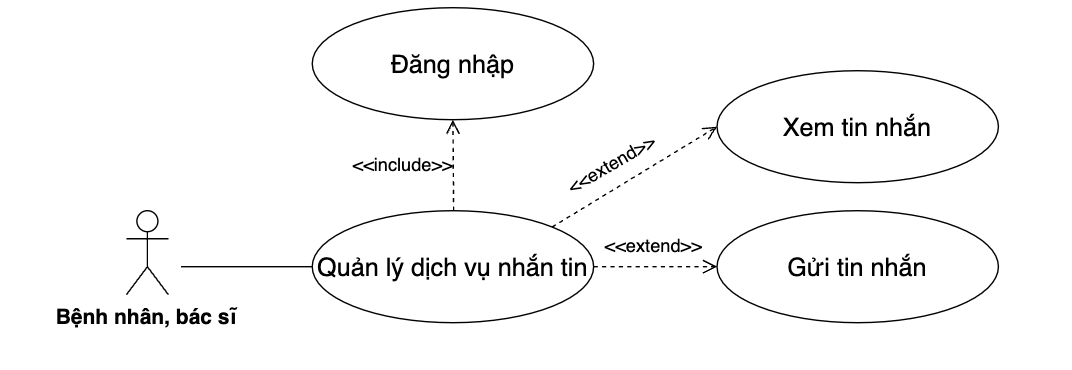
\includegraphics[width=15cm,height=6cm]{Images/mobile_app/use_case_send_receive_message.png}
    \caption[Sơ đồ tuần tự chức năng đăng ký trên App]{\bfseries \fontsize{12pt}{0pt}
    \selectfont Sơ đồ tuần tự chức năng đăng ký trên App}
    \label{hinh21} %đặt tên cho ảnh
  \end{figure}

  \begin{figure}[H]
    \centering
    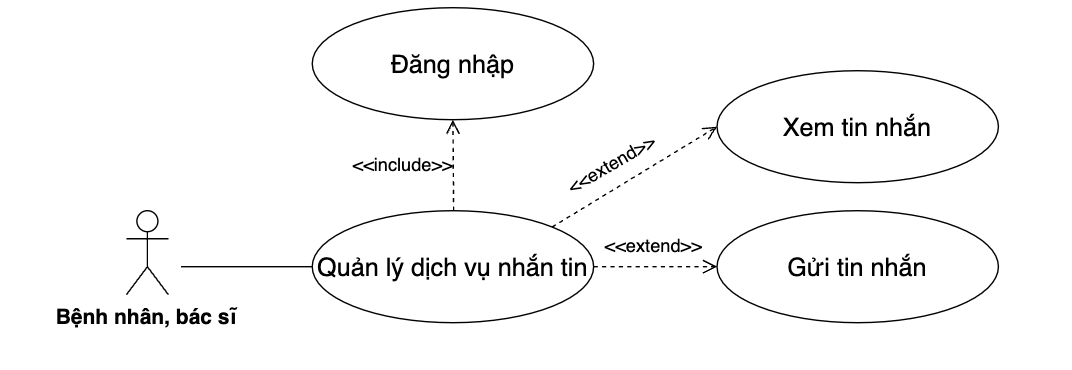
\includegraphics[width=15cm,height=6cm]{Images/mobile_app/use_case_send_receive_message.png}
    \caption[Sơ đồ tuần tự chức năng đăng ký trên App]{\bfseries \fontsize{12pt}{0pt}
    \selectfont Sơ đồ tuần tự chức năng đăng ký trên App}
    \label{hinh21} %đặt tên cho ảnh
  \end{figure}

  \begin{figure}[H]
    \centering
    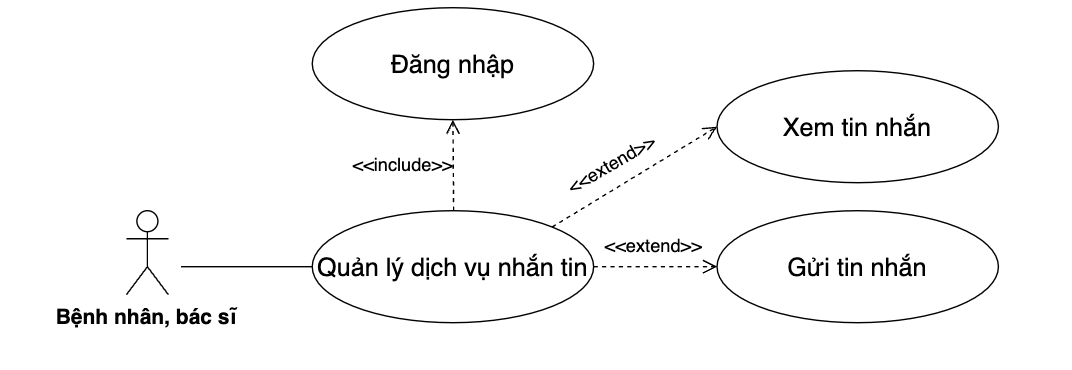
\includegraphics[width=15cm,height=6cm]{Images/mobile_app/use_case_send_receive_message.png}
    \caption[Sơ đồ tuần tự chức năng đăng ký trên App]{\bfseries \fontsize{12pt}{0pt}
    \selectfont Sơ đồ tuần tự chức năng đăng ký trên App}
    \label{hinh21} %đặt tên cho ảnh
  \end{figure}

  \begin{figure}[H]
    \centering
    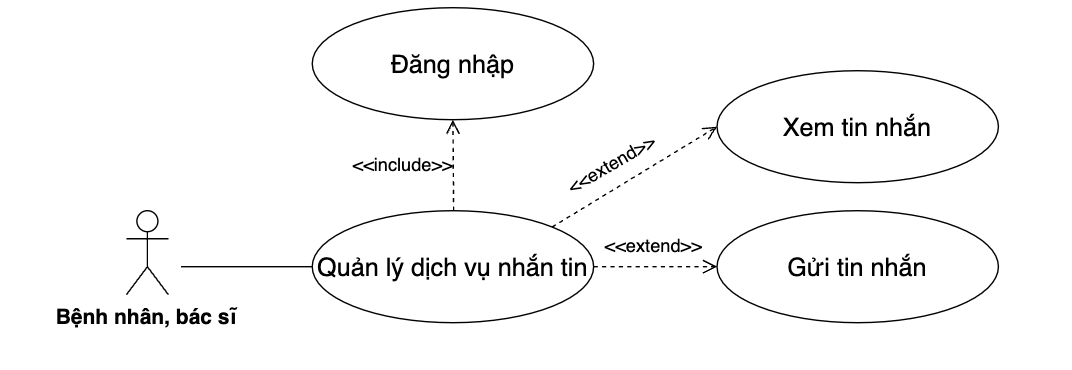
\includegraphics[width=15cm,height=6cm]{Images/mobile_app/use_case_send_receive_message.png}
    \caption[Sơ đồ tuần tự chức năng đăng ký trên App]{\bfseries \fontsize{12pt}{0pt}
    \selectfont Sơ đồ tuần tự chức năng đăng ký trên App}
    \label{hinh21} %đặt tên cho ảnh
  \end{figure}


\subsubsection{Sơ đồ kiến trúc hệ thống}

\begin{figure}[H]
  \centering
  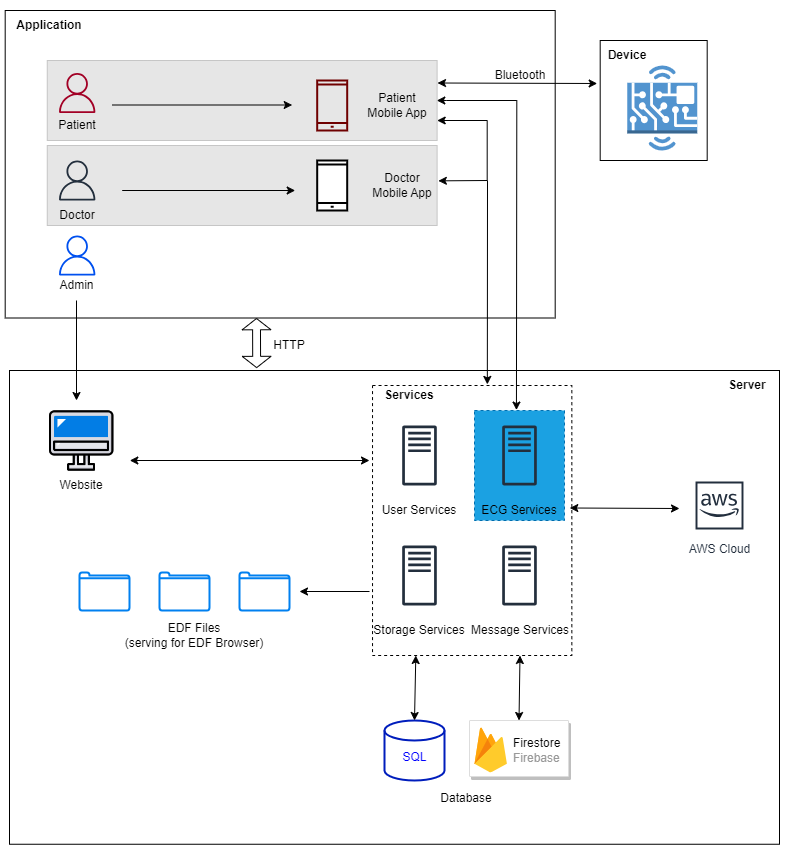
\includegraphics[width=16cm,height=18cm]{Images/system/fmECG_architecture-System Architecture.drawio.png}
  \caption[Kiến trúc hệ thống]{\bfseries \fontsize{12pt}{0pt}\selectfont Kiến trúc hệ thống}
  \label{hinh15} %đặt tên cho ảnh
\end{figure}

\subsubsection{Sơ đồ khối phần mềm}

\paragraph{Ứng dụng cho bệnh nhân}
\mbox{}

\begin{figure}[H]
  \centering
  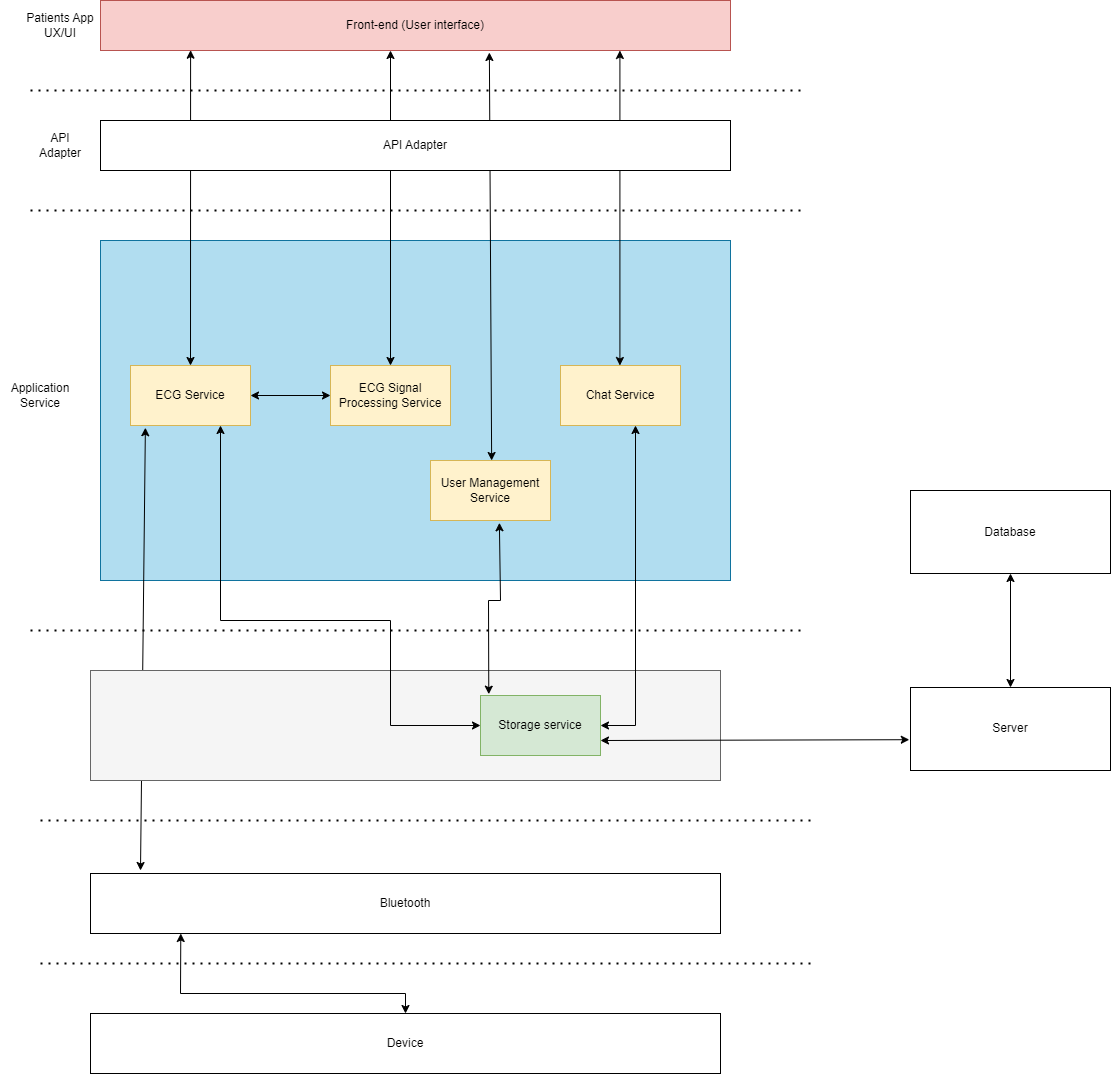
\includegraphics[width=16cm,height=18cm]{Images/system/fmECG_architecture-Patient.drawio.png}
  \caption[Kiến trúc hệ thống]{\bfseries \fontsize{12pt}{0pt}\selectfont Kiến trúc hệ thống}
  \label{hinh15} %đặt tên cho ảnh
\end{figure}

\paragraph{Ứng dụng cho bác sỹ}
\mbox{}


\begin{figure}[H]
  \centering
  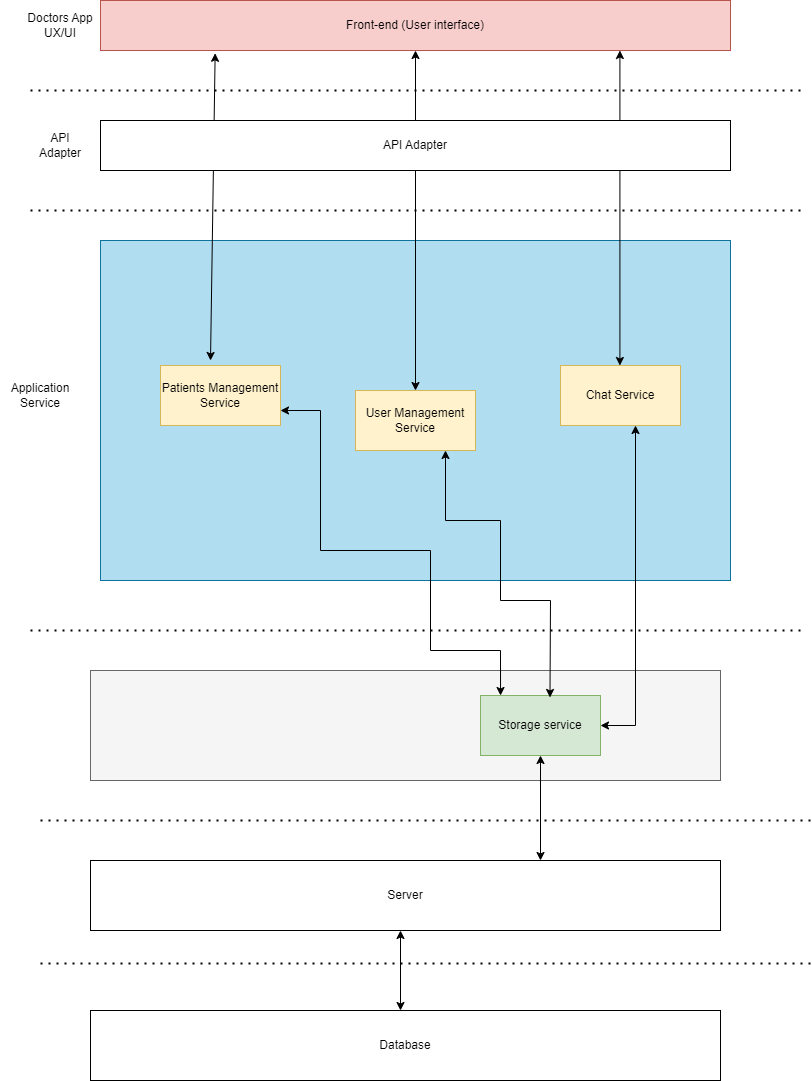
\includegraphics[width=16cm,height=18cm]{Images/system/fmECG_architecture-Doctors.drawio.png}
  \caption[Kiến trúc hệ thống]{\bfseries \fontsize{12pt}{0pt}\selectfont Kiến trúc hệ thống}
  \label{hinh15} %đặt tên cho ảnh
\end{figure}


\paragraph{Website cho admin}
\mbox{}

\begin{figure}[H]
  \centering
  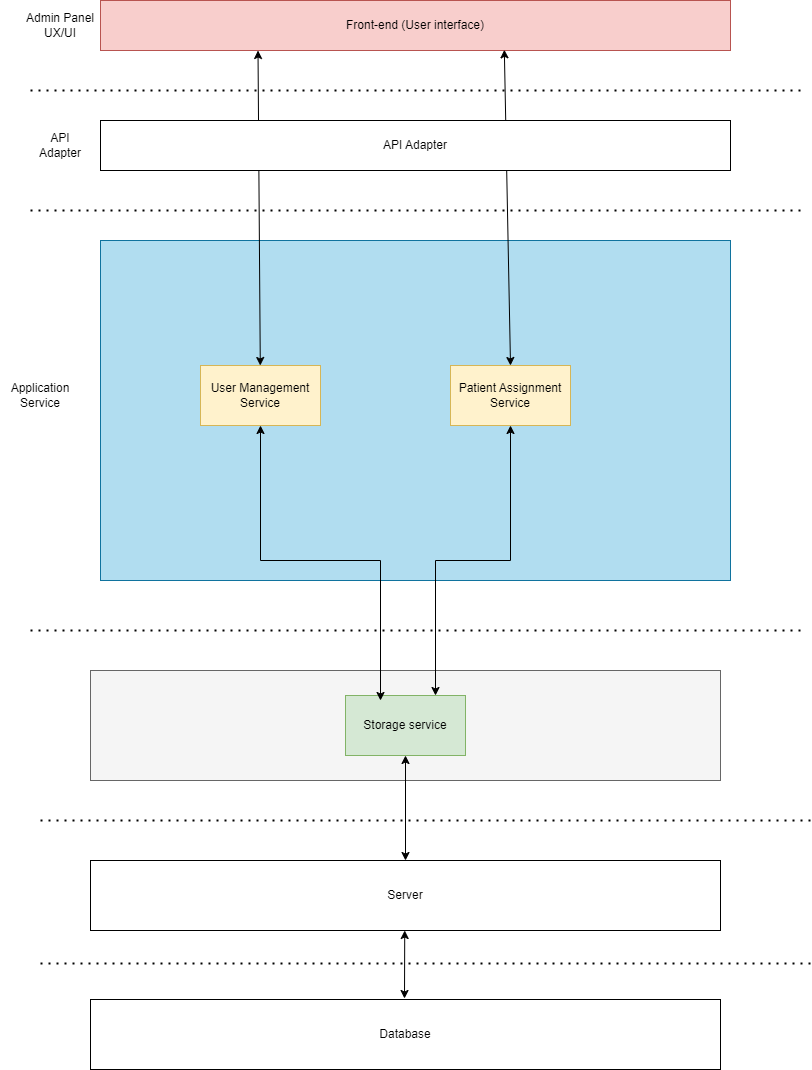
\includegraphics[width=16cm,height=18cm]{Images/system/fmECG_architecture-Admin.drawio.png}
  \caption[Kiến trúc hệ thống]{\bfseries \fontsize{12pt}{0pt}\selectfont Kiến trúc hệ thống}
  \label{hinh15} %đặt tên cho ảnh
\end{figure}

\subsubsection{Sơ đồ tuần tự}

\paragraph{Sơ đồ tuần tự chức năng đăng ký}
\mbox{}

    \begin{figure}[H]
         \centering
         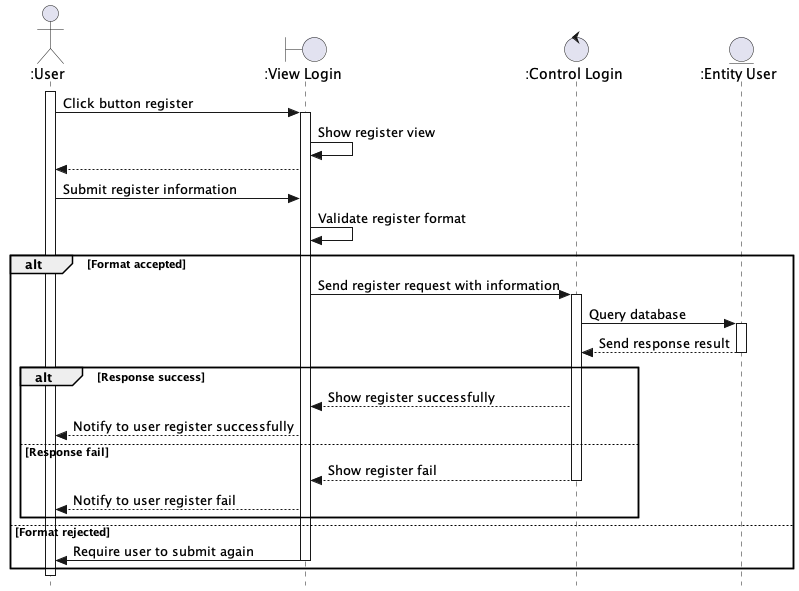
\includegraphics[width=16cm,height=12cm]{Images/mobile_app/register.png}
         \caption[Sơ đồ tuần tự chức năng đăng ký trên App]{\bfseries \fontsize{12pt}{0pt}
         \selectfont Sơ đồ tuần tự chức năng đăng ký trên App}
         \label{hinh21} %đặt tên cho ảnh
    \end{figure}

\paragraph{Sơ đồ tuần tự chức năng đăng nhập}
\mbox{}

    \begin{figure}[H]
         \centering
         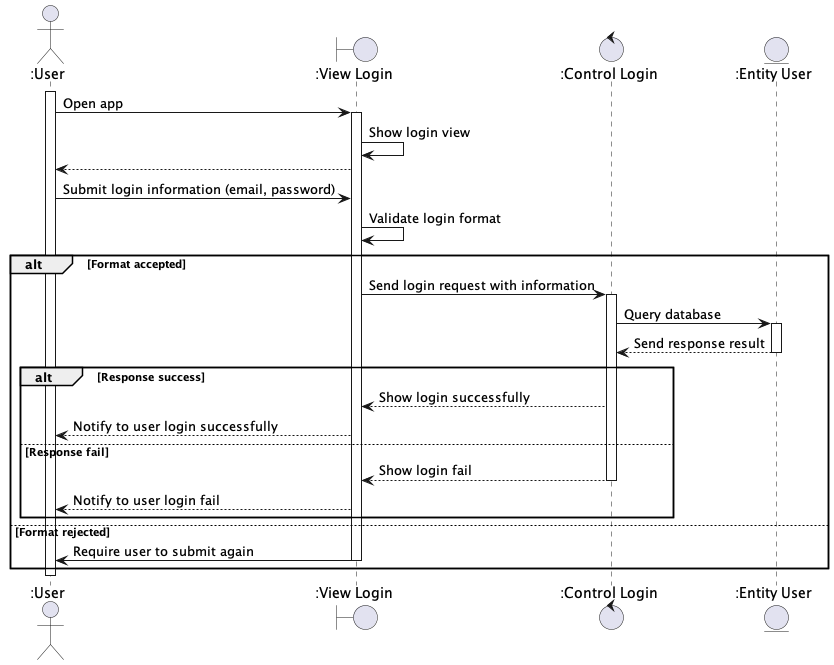
\includegraphics[width=16cm,height=12cm]{Images/mobile_app/login.png}
         \caption[Sơ đồ tuần tự chức năng đăng nhập trên App]{\bfseries \fontsize{12pt}{0pt}
         \selectfont Sơ đồ tuần tự chức năng đăng nhập trên App}
         \label{hinh21} %đặt tên cho ảnh
    \end{figure}

\paragraph{Sơ đồ tuần tự chức năng quên mật khẩu}
\mbox{}

    \begin{figure}[H]
         \centering
         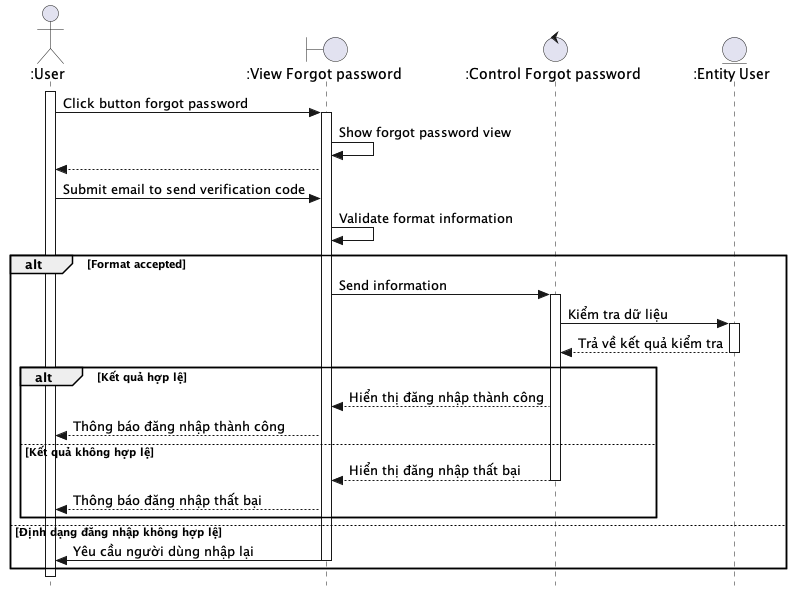
\includegraphics[width=16cm,height=12cm]{Images/mobile_app/forgot_password.png}
         \caption[Sơ đồ tuần tự chức năng quên mật khẩu trên App]{\bfseries \fontsize{12pt}{0pt}
         \selectfont Sơ đồ tuần tự chức năng quên mật khẩu trên App}
         \label{hinh21} %đặt tên cho ảnh
    \end{figure}

\paragraph{Sơ đồ tuần tự chức năng xem lịch sử các lần đo}
\mbox{}


    \begin{figure}[H]
         \centering
         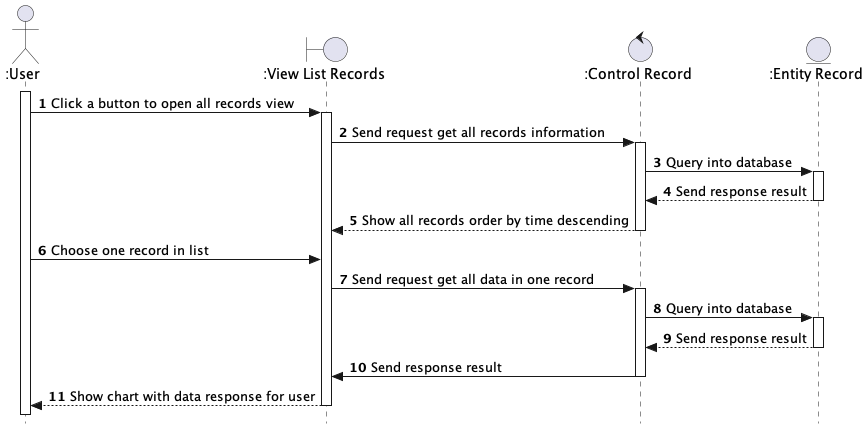
\includegraphics[width=16cm,height=11cm]{Images/mobile_app/view_record_timeline.png}
         \caption[Sơ đồ tuần tự chức năng xem lịch sử các lần đo trên App]{\bfseries \fontsize{12pt}{0pt}
         \selectfont Sơ đồ tuần tự chức năng xem lịch sử các lần đo trên App}
         \label{hinh21} %đặt tên cho ảnh
    \end{figure}

\paragraph{Sơ đồ tuần tự chức năng xem thay đổi thông tin cá nhân}
\mbox{}

  \begin{figure}[H]
        \centering
        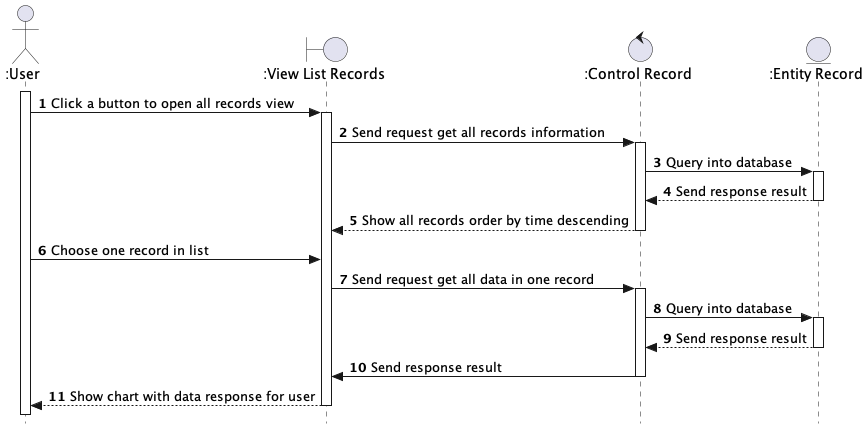
\includegraphics[width=16cm,height=11cm]{Images/mobile_app/view_record_timeline.png}
        \caption[Sơ đồ tuần tự chức năng xem thay đổi thông tin cá nhân trên App]{\bfseries \fontsize{12pt}{0pt}
        \selectfont Sơ đồ tuần tự chức năng xem thay đổi thông tin cá nhân trên App}
        \label{hinh21} %đặt tên cho ảnh
  \end{figure}

  \paragraph{Sơ đồ tuần tự chức năng đổi mật khẩu}
\mbox{}

  \begin{figure}[H]
        \centering
        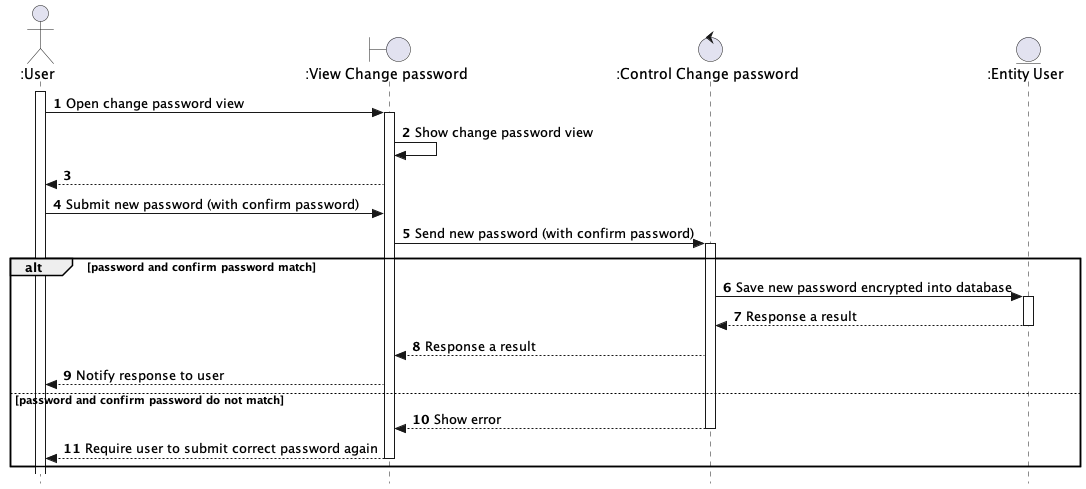
\includegraphics[width=16cm,height=11cm]{Images/mobile_app/change_password.png}
        \caption[Sơ đồ tuần tự chức năng đổi mật khẩu trên App]{\bfseries \fontsize{12pt}{0pt}
        \selectfont Sơ đồ tuần tự chức năng đổi mật khẩu trên App}
        \label{hinh21} %đặt tên cho ảnh
  \end{figure}


\paragraph{Sơ đồ tuần tự chức năng xem/gửi tin nhắn}
\mbox{}

  \begin{figure}[H]
        \centering
        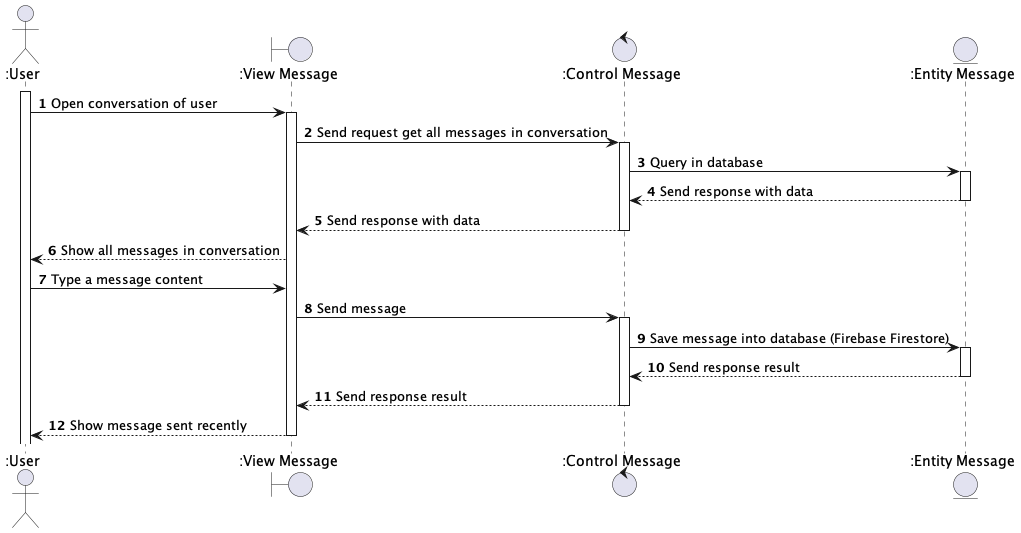
\includegraphics[width=16cm,height=11cm]{Images/mobile_app/send_and_receive_message.png}
        \caption[Sơ đồ tuần tự chức năng xem/gửi tin nhắn trên App]{\bfseries \fontsize{12pt}{0pt}
        \selectfont Sơ đồ tuần tự chức năng xem/gửi tin nhắn trên App}
        \label{hinh21} %đặt tên cho ảnh
  \end{figure}


\paragraph{Sơ đồ tuần tự chức năng xem bài đăng tin tức}
\mbox{}

  \begin{figure}[H]
        \centering
        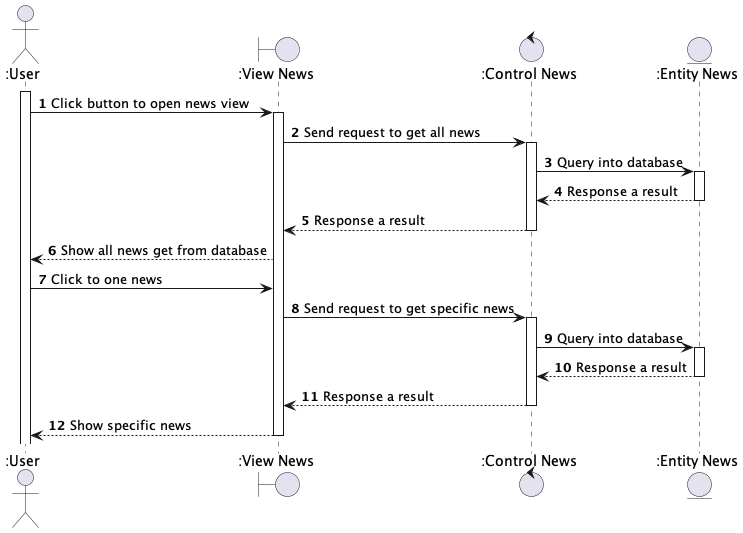
\includegraphics[width=16cm,height=11cm]{Images/mobile_app/view_news.png}
        \caption[ Sơ đồ tuần tự chức năng xem bài đăng tin tứctrên App]{\bfseries \fontsize{12pt}{0pt}
        \selectfont Sơ đồ tuần tự chức năng xem bài đăng tin tức trên App}
        \label{hinh21} %đặt tên cho ảnh
  \end{figure}

\paragraph{Sơ đồ tuần tự chức năng bật/tắt Bluetooth}
\mbox{}

  \begin{figure}[H]
        \centering
        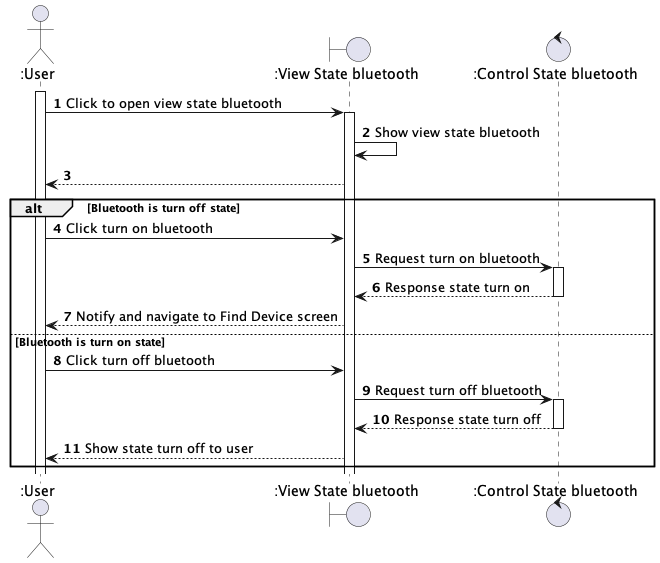
\includegraphics[width=16cm,height=12cm]{Images/mobile_app/turn_on_off_bluetooth.png}
        \caption[Sơ đồ tuần tự chức năng bật/tắt Bluetooth trên App]{\bfseries \fontsize{12pt}{0pt}
        \selectfont Sơ đồ tuần tự chức năng bật/tắt Bluetooth trên App}
        \label{hinh21} %đặt tên cho ảnh
  \end{figure}


\paragraph{Sơ đồ tuần tự chức năng kết nối Bluetooth với thiết bị đo điện tim}
\mbox{}

  \begin{figure}[H]
        \centering
        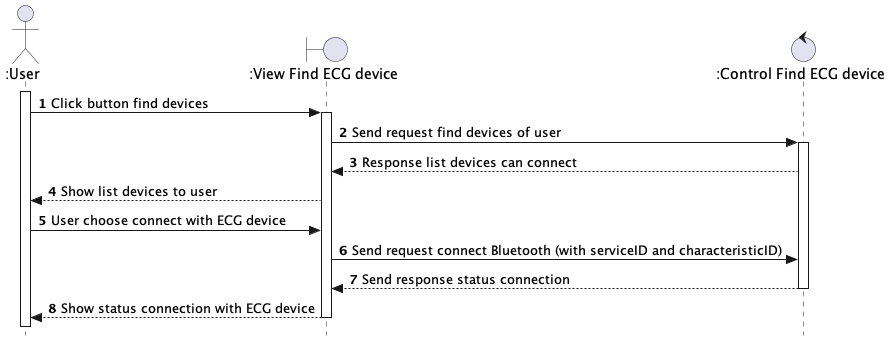
\includegraphics[width=16cm,height=10cm]{Images/mobile_app/connect_with_device.png}
        \caption[Sơ đồ tuần tự chức năng kết nối Bluetooth với thiết bị đo điện tim trên App]{\bfseries \fontsize{12pt}{0pt}
        \selectfont Sơ đồ tuần tự chức năng kết nối Bluetooth với thiết bị đo điện tim trên App}
        \label{hinh21} %đặt tên cho ảnh
  \end{figure}



\paragraph{Sơ đồ tuần tự chức năng ngắt kết nối Bluetooth với thiết bị đo điện tim}
\mbox{}

  \begin{figure}[H]
        \centering
        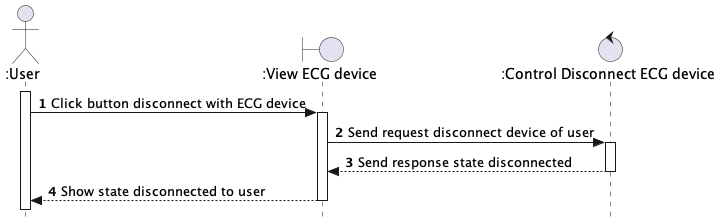
\includegraphics[width=16cm,height=9cm]{Images/mobile_app/disconnect_with_device.png}
        \caption[Sơ đồ tuần tự chức năng ngắt kết nối Bluetooth với thiết bị đo điện tim trên App]{\bfseries \fontsize{12pt}{0pt}
        \selectfont Sơ đồ tuần tự chức năng ngắt kết nối Bluetooth với thiết bị đo điện tim trên App}
        \label{hinh21} %đặt tên cho ảnh
  \end{figure}


\paragraph{Sơ đồ tuần tự chức năng tiến hành đo điện tim}
\mbox{}

  \begin{figure}[H]
        \centering
        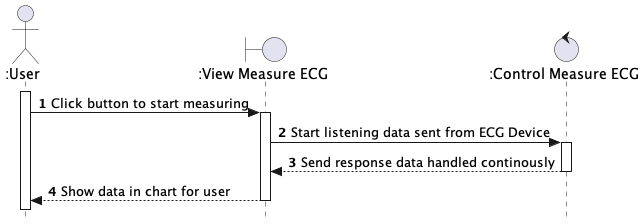
\includegraphics[width=16cm,height=9cm]{Images/mobile_app/start_measuring_ecg.png}
        \caption[Sơ đồ tuần tự chức năng tiến hành đo điện tim trên App]{\bfseries \fontsize{12pt}{0pt}
        \selectfont Sơ đồ tuần tự chức năng tiến hành đo điện tim trên App}
        \label{hinh21} %đặt tên cho ảnh
  \end{figure}
 

\paragraph{Sơ đồ tuần tự chức năng kết thúc quá trình đo điện tim}
\mbox{}

  \begin{figure}[H]
        \centering
        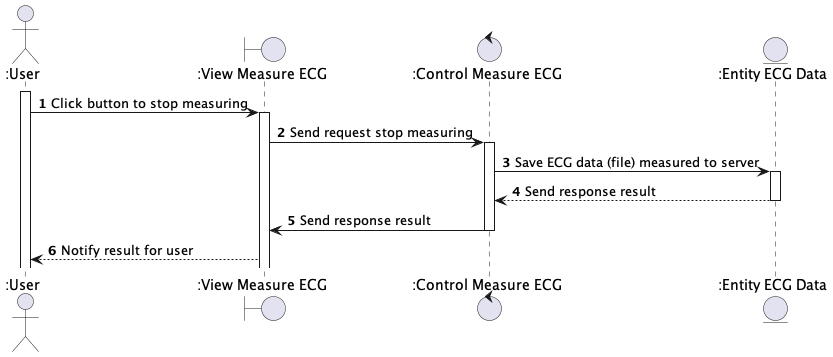
\includegraphics[width=16cm,height=9cm]{Images/mobile_app/end_measuring_ecg.png}
        \caption[Sơ đồ tuần tự chức năng kết thúc quá trình đo điện tim trên App]{\bfseries \fontsize{12pt}{0pt}
        \selectfont Sơ đồ tuần tự chức năng kết thúc quá trình đo điện tim trên App}
        \label{hinh21} %đặt tên cho ảnh
  \end{figure}





\newpage

\section*{CHƯƠNG 2. THIẾT KẾ CHI TIẾT HỆ THỐNG}
\setcounter{section}{2}
\setcounter{subsection}{0} %LƯU Ý MỖI LẦN THÊM CHƯƠNG MỚI CẦN THÊM CÂU NÀY ĐỂ RESET THỨ TỰ CỦA SUBSECTON VỀ 1
\setcounter{table}{0} % LƯU Ý SAU MỖI LẦN GỌI BẢNG HAY HÌNH ẢNH PHẢI THÊM CÂU NÀY ĐỂ RESET THỨ TỰ
\setcounter{figure}{0} %% LƯU Ý SAU MỖI LẦN GỌI BẢNG HAY HÌNH ẢNH PHẢI THÊM CÂU NÀY ĐỂ RESET THỨ TỰ
\addcontentsline{toc}{section}{\numberline{}CHƯƠNG 2. THIẾT KẾ CHI TIẾT HỆ THỐNG}

\subsection{Công nghệ sử dụng}



\subsection{Thiết kế cơ sở dữ liệu}

\subsubsection{Xây dựng mô hình thực thể liên kết}

Xác định các thực thể và thuộc tính:


\begin{table}[H]
  \caption{\bfseries \fontsize{12pt}{0pt}\selectfont Bảng thực thể và thuộc tính}
  \centering
  \begin{tabularx}{0.9\textwidth}{|c|X|}
    \hline
    \textbf{Thực thể} & \textbf{Thuộc tính} \\
    \hline
    Người dùng & 
    ID người dùng, Mật khẩu, Email, Tên, Ngày sinh, Số điện thoại, Quyền \\
    \hline
    ECG Record & 
    ID bản ghi ECG, ID người dùng, ID thiết bị, Đường dẫn lưu trữ dữ liệu, Thời gian bắt đầu, Thời gian kết thúc, Loại cảm biến \\
    \hline
    Danh mục tin tức & 
    ID danh mục tin tức, Tên danh mục tin tức, Mô tả danh mục tin tức \\
    \hline
    Tin tức & 
    ID tin tức, Tiêu đề, Nội dung, ID danh mục tin tức, Tác giả, Đường dẫn, Đường dẫn hình ảnh \\
    \hline
    Phân công bệnh nhân - bác sĩ & 
    ID phân công, ID bệnh nhân, ID bác sĩ, Ngày bắt đầu \\
    \hline
    Mã thông báo đặt lại & 
    ID mã thông báo, ID người dùng, Mã thông báo, Thời gian hết hạn \\
    \hline
    Phiên đăng nhập & 
    ID phiên đăng nhập, ID người dùng, Mã phiên đăng nhập, Thời gian hết hạn \\
    \hline
    Thiết bị & 
    ID thiết bị, Tên thiết bị \\
    \hline
  \end{tabularx}
\end{table}



\subsubsection{Chuyển mô hình thực thể liên kết sang mô hình quan hệ}
Các bảng trong mô hình thực thể liên kết đã được chuyển thành các bảng trong mô hình quan hệ, với mỗi bảng đại diện cho một thực thể và các mối quan hệ được biểu diễn bằng các khóa ngoại.

\subsubsection{Mối quan hệ dữ liệu}

\begin{itemize}
  \item Bảng \texttt{ecg\_record} có mối quan hệ 1-n với bảng \texttt{user} thông qua khóa ngoại \texttt{user\_id}.
  \item Bảng \texttt{news} có mối quan hệ n-1 với bảng \texttt{news\_category} thông qua khóa ngoại \texttt{category\_id}.
  \item Bảng \texttt{patient\_doctor\_assignment} có mối quan hệ n-1 với bảng \texttt{user} thông qua khóa ngoại \texttt{patient\_id} và \texttt{doctor\_id}.
  \item Bảng \texttt{reset\_token} có mối quan hệ n-1 với bảng \texttt{user} thông qua khóa ngoại \texttt{user\_id}.
\end{itemize}

\subsubsection{Chuẩn hoá 3NF}
Các bảng đã được thiết kế theo nguyên tắc chuẩn hoá 3NF, vì không có thuộc tính lặp lại và các thuộc tính không phụ thuộc vào một tập hợp con của khóa chính.
\subsubsection{Từ điển dữ liệu}



\begin{table}[H]
  \caption{\bfseries \fontsize{12pt}{0pt}\selectfont Bảng \texttt{user}}
  \centering
  \begin{tabularx}{0.9\textwidth}{|c|c|X|}
    \hline
    \textbf{Thuộc tính} & \textbf{Kiểu dữ liệu} & \textbf{Mô tả} \\
    \hline
    user\_id & INTEGER & Khóa chính của bảng, đại diện cho ID người dùng. \\
    \hline
    password & STRING & Mật khẩu của người dùng. \\
    \hline
    email & STRING & Địa chỉ email của người dùng. \\
    \hline
    name & STRING & Tên của người dùng. \\
    \hline
    doB & DATE & Ngày sinh của người dùng. \\
    \hline
    phone\_number & STRING & Số điện thoại của người dùng. \\
    \hline
    role & INTEGER & Quyền của người dùng (0-patient, 1-doctor, 2-admin). \\
    \hline
  \end{tabularx}
\end{table}

\begin{table}[H]
  \caption{\bfseries \fontsize{12pt}{0pt}\selectfont Bảng \texttt{ecg\_record}}
  \centering
  \begin{tabularx}{0.9\textwidth}{|c|c|X|}
    \hline
    \textbf{Thuộc tính} & \textbf{Kiểu dữ liệu} & \textbf{Mô tả} \\
    \hline
    record\_id & INTEGER & Khóa chính của bảng, đại diện cho ID bản ghi ECG. \\
    \hline
    user\_id & INTEGER & Khóa ngoại tham chiếu đến \texttt{user\_id} trong bảng \texttt{user}. \\
    \hline
    device\_id & STRING & ID thiết bị. \\
    \hline
    data\_directory & STRING & Đường dẫn lưu trữ dữ liệu. \\
    \hline
    start\_time & DATE & Thời gian bắt đầu ghi lại ECG. \\
    \hline
    stop\_time & DATE & Thời gian kết thúc ghi lại ECG. \\
    \hline
    sensor\_type & STRING & Loại cảm biến. \\
    \hline
  \end{tabularx}
\end{table}

\begin{table}[H]
  \caption{\bfseries \fontsize{12pt}{0pt}\selectfont Bảng \texttt{news\_category}}
  \centering
  \begin{tabularx}{0.9\textwidth}{|c|c|X|}
    \hline
    \textbf{Thuộc tính} & \textbf{Kiểu dữ liệu} & \textbf{Mô tả} \\
    \hline
    category\_id & INTEGER & Khóa chính của bảng, đại diện cho ID danh mục tin tức. \\
    \hline
    category\_name & STRING & Tên danh mục tin tức. \\
    \hline
    category\_description & STRING & Mô tả danh mục tin tức. \\
    \hline
  \end{tabularx}
\end{table}

\begin{table}[H]
  \caption{\bfseries \fontsize{12pt}{0pt}\selectfont Bảng \texttt{news}}
  \centering
  \begin{tabularx}{0.9\textwidth}{|c|c|X|}
    \hline
    \textbf{Thuộc tính} & \textbf{Kiểu dữ liệu} & \textbf{Mô tả} \\
    \hline
    news\_id & INTEGER & Khóa chính của bảng, đại diện cho ID tin tức. \\
    \hline
    title & STRING & Tiêu đề tin tức. \\
    \hline
    content & TEXT & Nội dung tin tức. \\
    \hline
    category\_id & INTEGER & Khóa ngoại tham chiếu đến \texttt{category\_id} trong bảng \texttt{news\_category}. \\
    \hline
    author & STRING & Tác giả tin tức. \\
    \hline
    url & STRING & Đường dẫn tin tức. \\
    \hline
    image & STRING & Đường dẫn hình ảnh tin tức (có thể là null). \\
    \hline
  \end{tabularx}
\end{table}

\begin{table}[H]
  \caption{\bfseries \fontsize{12pt}{0pt}\selectfont Bảng \texttt{patient\_doctor\_assignment}}
  \centering
  \begin{tabularx}{0.9\textwidth}{|c|c|X|}
    \hline
    \textbf{Thuộc tính} & \textbf{Kiểu dữ liệu} & \textbf{Mô tả} \\
    \hline
    assign\_id & INTEGER & Khóa chính của bảng, đại diện cho ID phân công bệnh nhân - bác sĩ. \\
    \hline
    patient\_id & INTEGER & Khóa ngoại tham chiếu đến \texttt{user\_id} trong bảng \texttt{user} (với quyền là bệnh nhân). \\
    \hline
    doctor\_id & INTEGER & Khóa ngoại tham chiếu đến \texttt{user\_id} trong bảng \texttt{user} (với quyền là bác sĩ). \\
    \hline
    start\_date & DATE & Ngày bắt đầu phân công. \\
    \hline
  \end{tabularx}
\end{table}

\begin{table}[H]
  \caption{\bfseries \fontsize{12pt}{0pt}\selectfont Bảng \texttt{reset\_token}}
  \centering
  \begin{tabularx}{0.9\textwidth}{|c|c|X|}
    \hline
    \textbf{Thuộc tính} & \textbf{Kiểu dữ liệu} & \textbf{Mô tả} \\
    \hline
    id & INTEGER & Khóa chính của bảng, đại diện cho ID mã thông báo đặt lại. \\
    \hline
    user\_id & INTEGER & Khóa ngoại tham chiếu đến \texttt{user\_id} trong bảng \texttt{user}. \\
    \hline
    token & STRING & Mã thông báo đặt lại. \\
    \hline
    expiration & DATE & Thời gian hết hạn của mã thông báo đặt lại. \\
    \hline
  \end{tabularx}
\end{table}


\begin{table}[H]
  \caption{\bfseries \fontsize{12pt}{0pt}\selectfont Bảng \texttt{session}}
  \centering
  \begin{tabularx}{0.9\textwidth}{|c|c|X|}
    \hline
    \textbf{Thuộc tính} & \textbf{Kiểu dữ liệu} & \textbf{Mô tả} \\
    \hline
    session\_id & INTEGER & Khóa chính của bảng, đại diện cho ID phiên đăng nhập. \\
    \hline
    user\_id & INTEGER & Khóa ngoại tham chiếu đến \texttt{user\_id} trong bảng \texttt{user}. \\
    \hline
    token & STRING & Mã phiên đăng nhập. \\
    \hline
    expiration & DATE & Thời gian hết hạn của phiên đăng nhập. \\
    \hline
  \end{tabularx}
\end{table}

\begin{table}[H]
  \caption{\bfseries \fontsize{12pt}{0pt}\selectfont Bảng \texttt{device}}
  \centering
  \begin{tabularx}{0.9\textwidth}{|c|c|X|}
    \hline
    \textbf{Thuộc tính} & \textbf{Kiểu dữ liệu} & \textbf{Mô tả} \\
    \hline
    device\_id & INTEGER & Khóa chính của bảng, đại diện cho ID thiết bị. \\
    \hline
    device\_name & STRING & Tên thiết bị. \\
    \hline
  \end{tabularx}
\end{table}

\subsection{Phân tích chi tiết hệ thống}

\subsubsection{Thiết kế giao diện}

\paragraph{Ứng dụng}
\mbox{}

\paragraph{Website}
\mbox{}

\subsubsection{Thiết kế API}


\subsubsection{Sơ đồ lớp}

\paragraph{Ứng dụng}
\mbox{}

\paragraph{Server và Website quản trị hệ thống}
\mbox{}

\begin{enumerate}[a)]
\item Danh sách các class diagram

\begin{figure}[H]
  \centering
  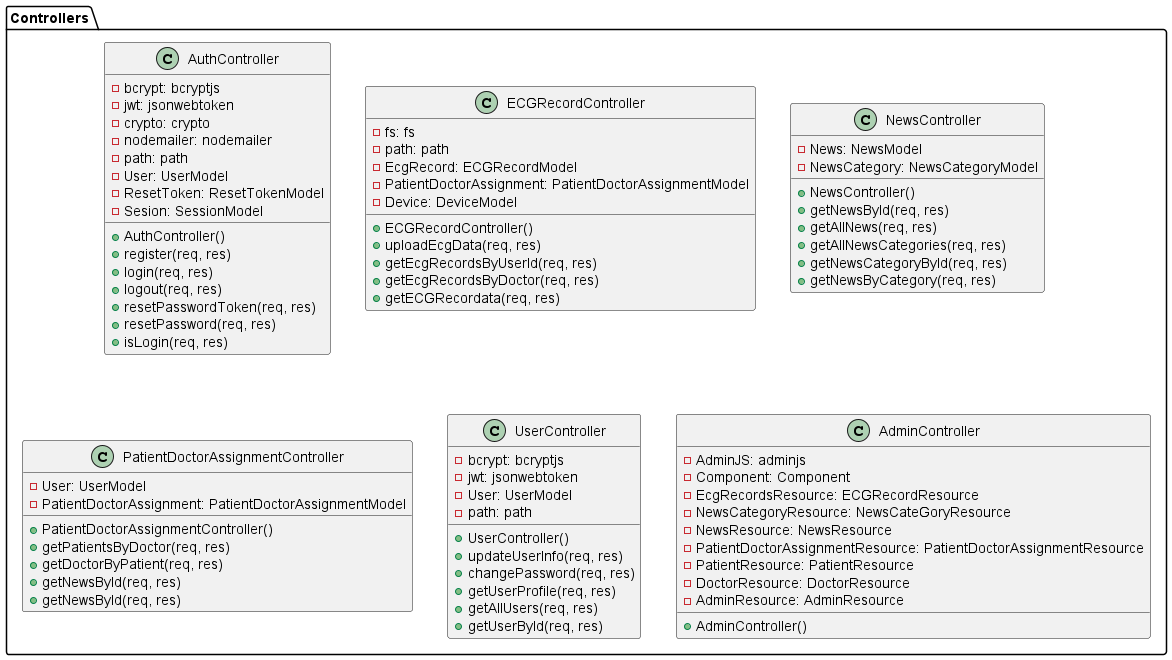
\includegraphics[width=15cm,height=12cm]{Images/server/class/class_controller.png}
  \caption[Sơ đồ lớp]{\bfseries \fontsize{12pt}{0pt}\selectfont Sơ đồ lớp}
  \label{hinh2} %đặt tên cho ảnh
\end{figure}



\begin{figure}[H]
  \centering
  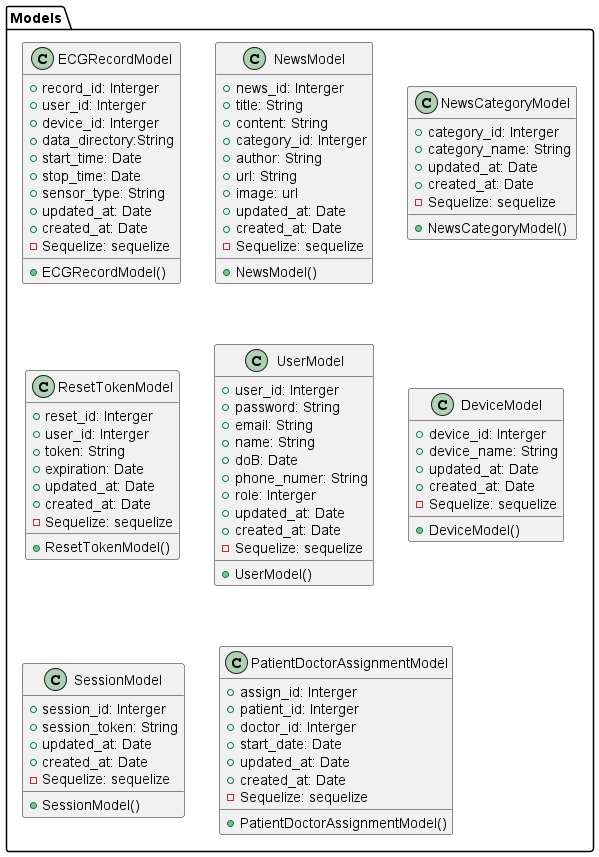
\includegraphics[width=15cm,height=12cm]{Images/server/class/class_model.png}
  \caption[Sơ đồ lớp]{\bfseries \fontsize{12pt}{0pt}\selectfont Sơ đồ lớp}
  \label{hinh2} %đặt tên cho ảnh
\end{figure}


\begin{figure}[H]
  \centering
  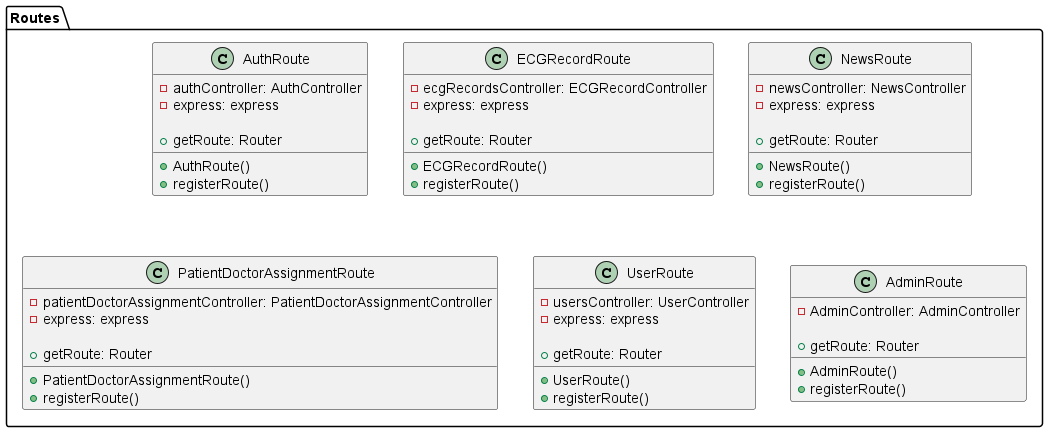
\includegraphics[width=15cm,height=12cm]{Images/server/class/class_route.png}
  \caption[Sơ đồ lớp]{\bfseries \fontsize{12pt}{0pt}\selectfont Sơ đồ lớp}
  \label{hinh2} %đặt tên cho ảnh
\end{figure}


\begin{figure}[H]
  \centering
  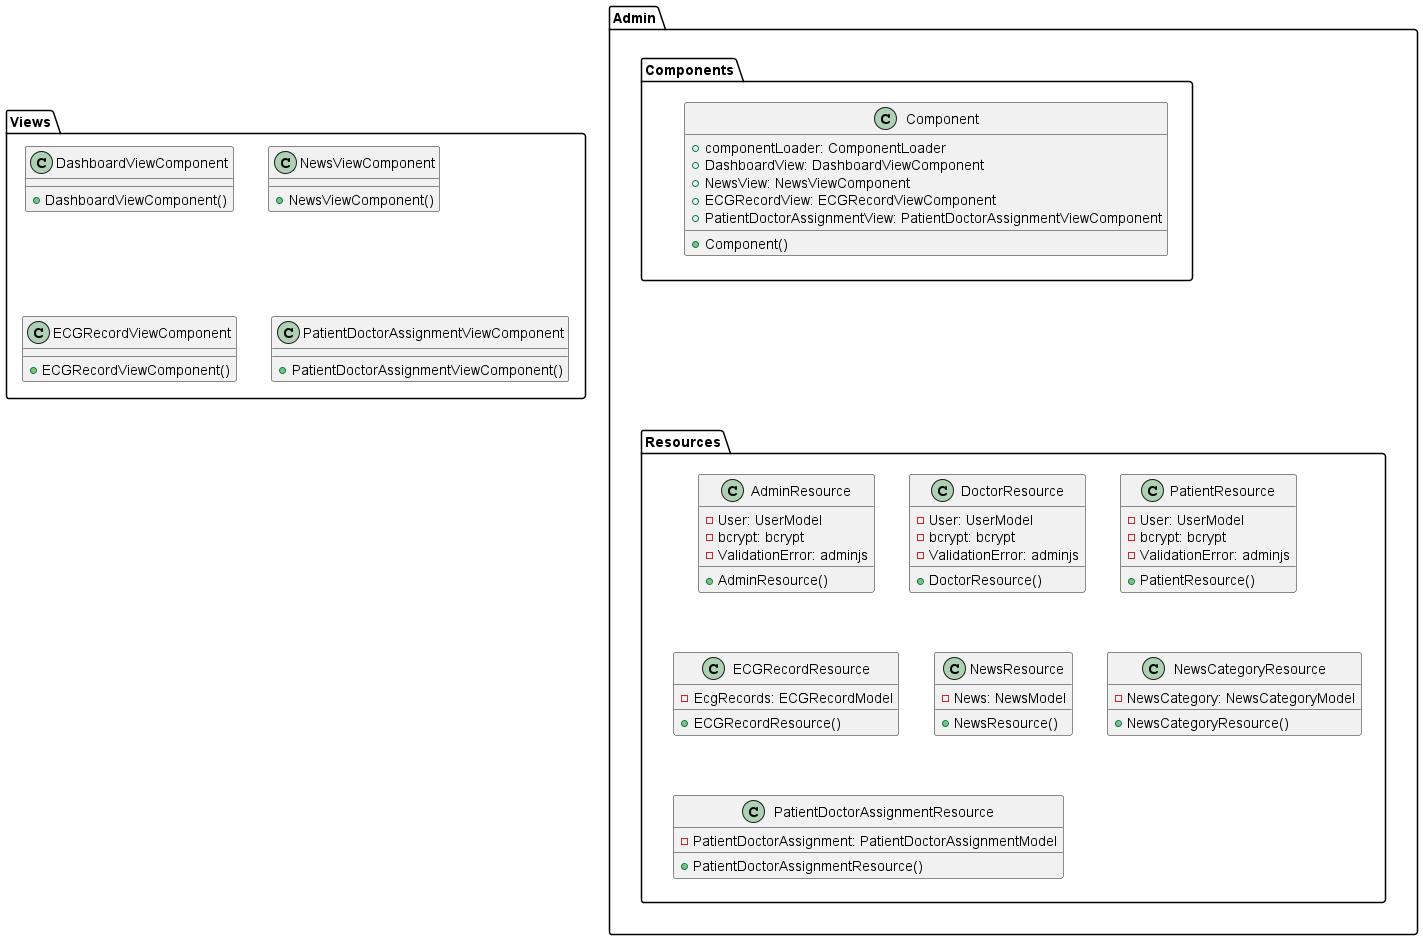
\includegraphics[width=15cm,height=12cm]{Images/server/class/class_admin.png}
  \caption[Sơ đồ lớp]{\bfseries \fontsize{12pt}{0pt}\selectfont Sơ đồ lớp}
  \label{hinh2} %đặt tên cho ảnh
\end{figure}


\item Mối quan hệ

\begin{figure}[H]
  \centering
  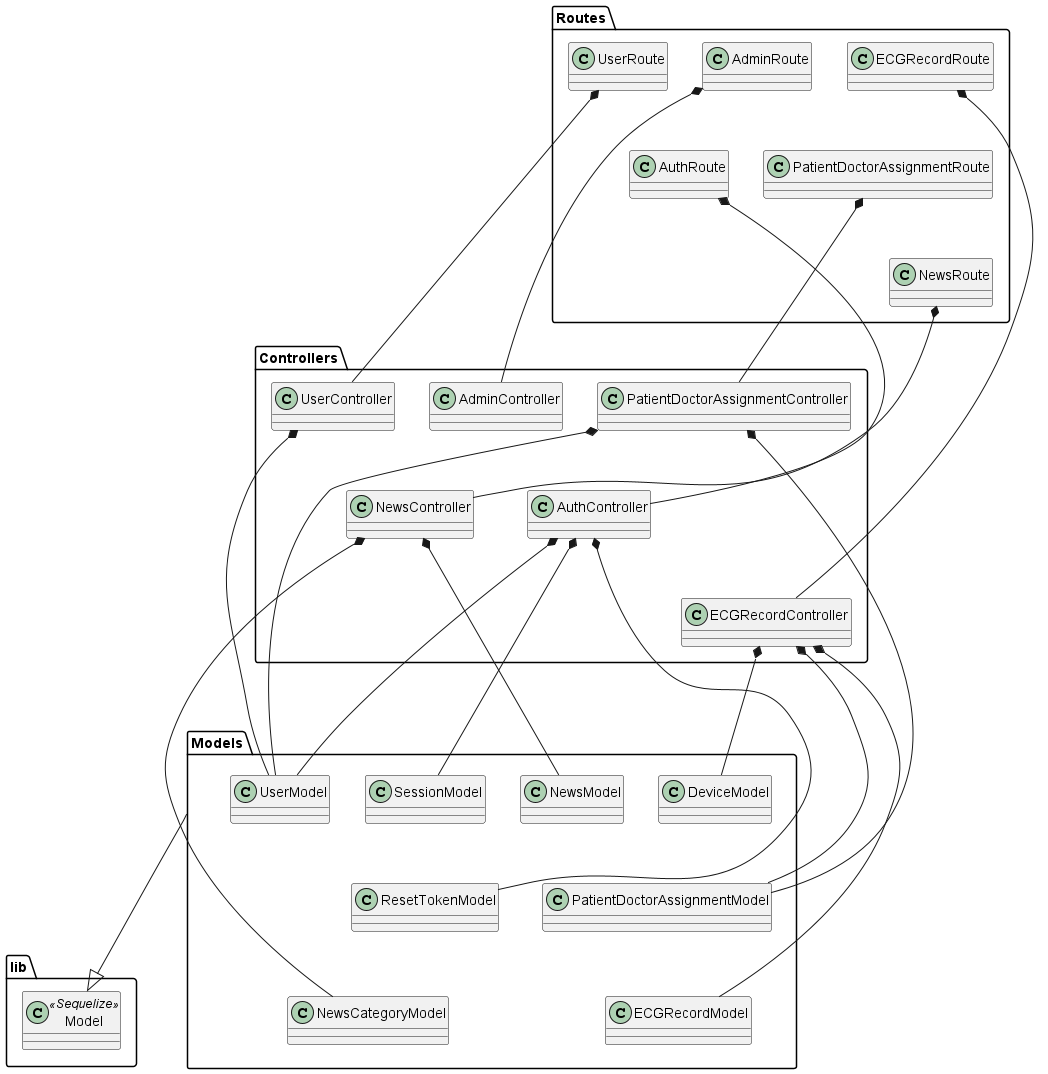
\includegraphics[width=15cm,height=12cm]{Images/server/class/class_relation.png}
  \caption[Sơ đồ lớp]{\bfseries \fontsize{12pt}{0pt}\selectfont Sơ đồ lớp}
  \label{hinh2} %đặt tên cho ảnh
\end{figure}


\begin{figure}[H]
  \centering
  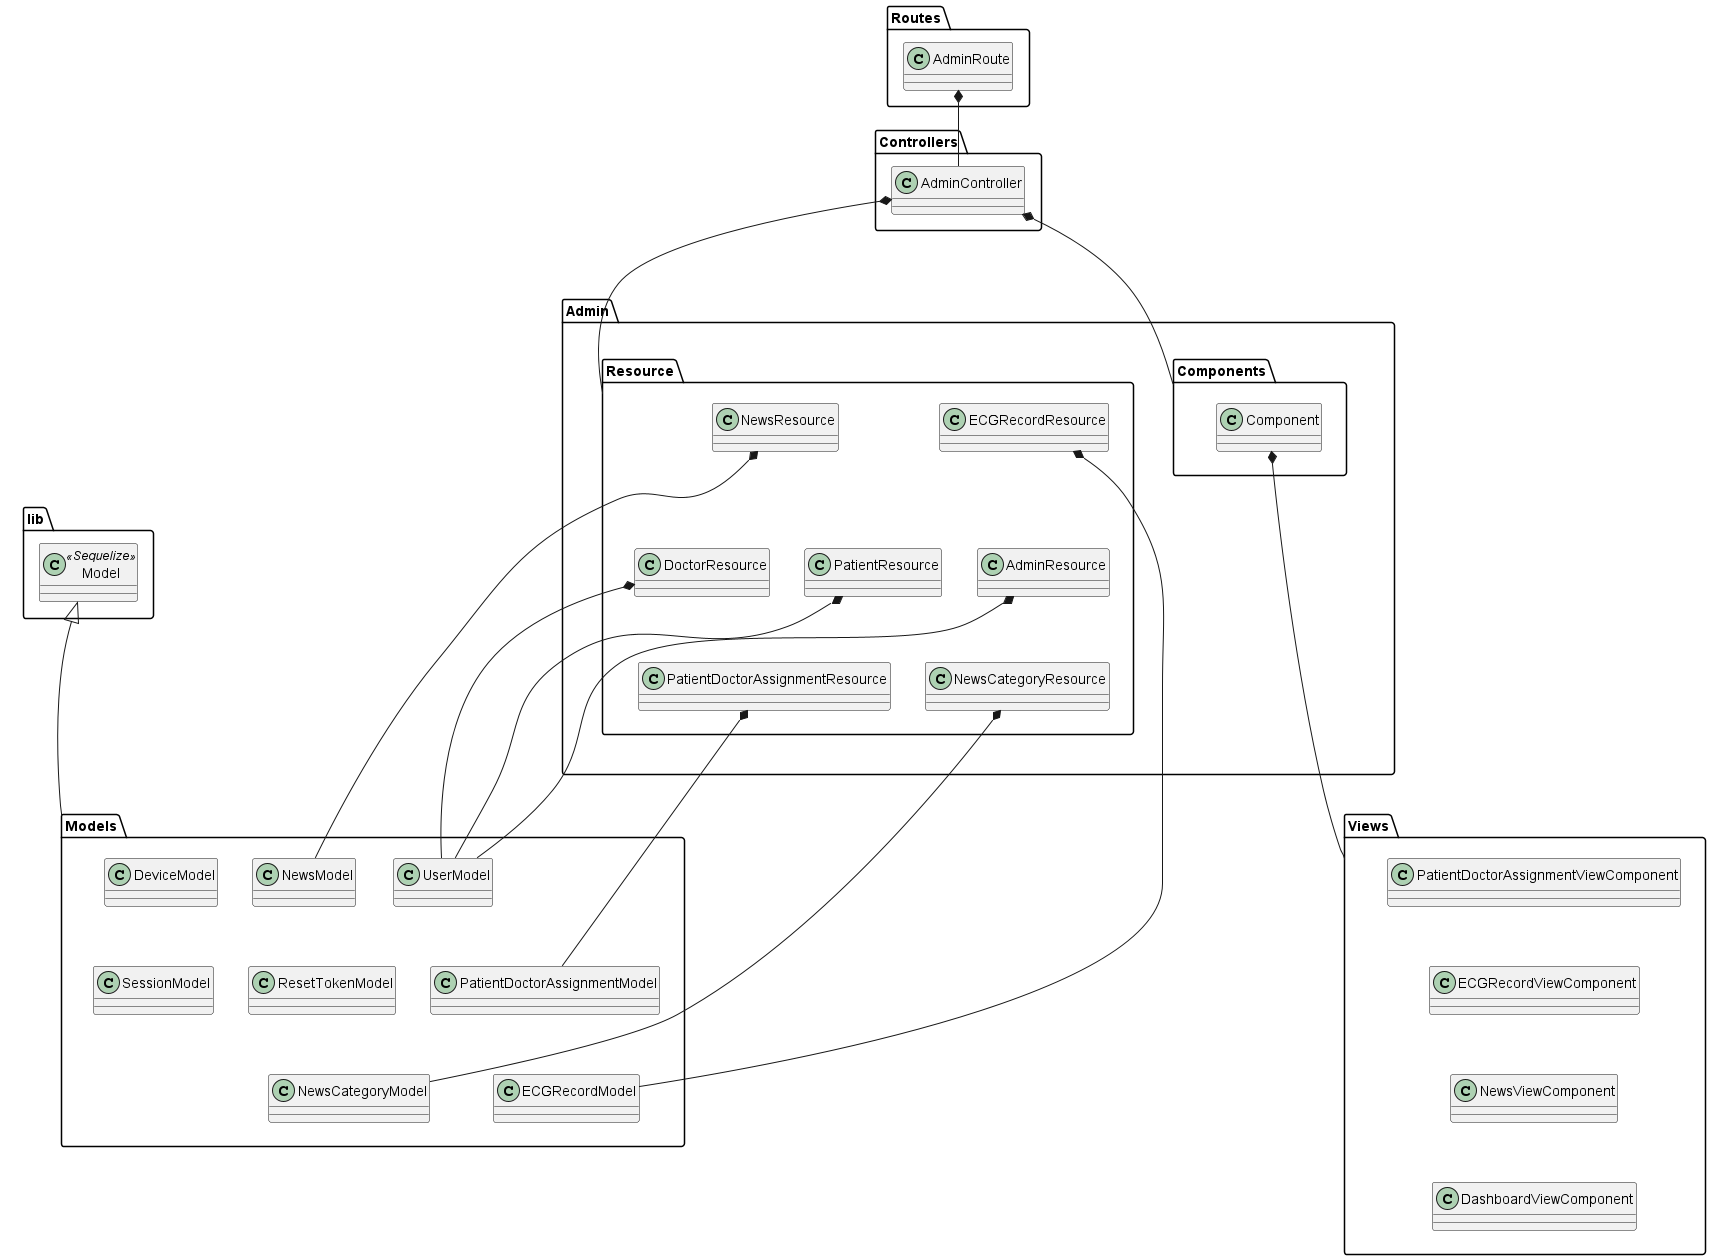
\includegraphics[width=15cm,height=12cm]{Images/server/class/class_admin_relation.png}
  \caption[Sơ đồ lớp]{\bfseries \fontsize{12pt}{0pt}\selectfont Sơ đồ lớp}
  \label{hinh2} %đặt tên cho ảnh
\end{figure}

\end{enumerate}


\subsubsection{Sơ đồ tuần tự}

\begin{figure}[H]
  \centering
  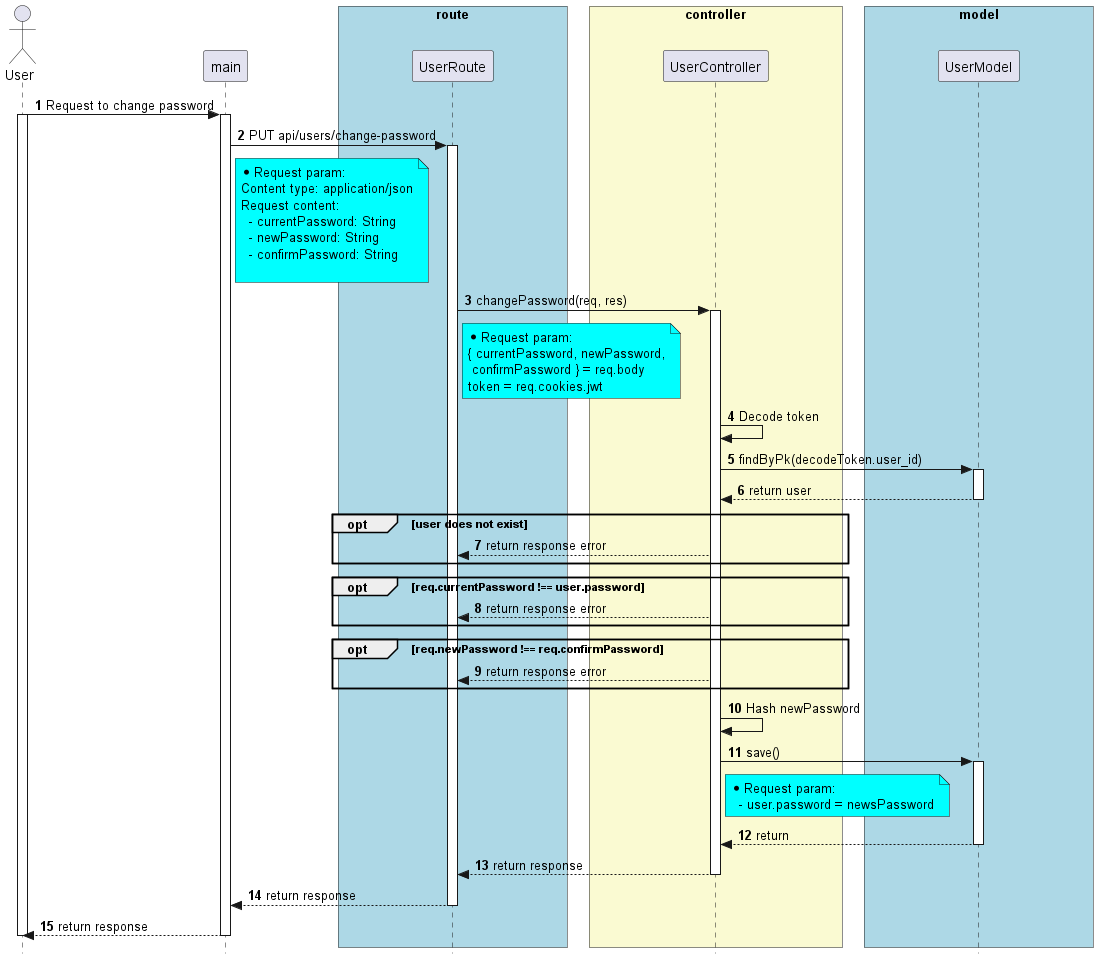
\includegraphics[width=16cm,height=9cm]{Images/server/sequence/server/changePassword.png}
  \caption[Sơ đồ tuần tự ]{\bfseries \fontsize{12pt}{0pt}
  \selectfont Sơ đồ tuần }
  \label{hinh21} %đặt tên cho ảnh
\end{figure}


\begin{figure}[H]
  \centering
  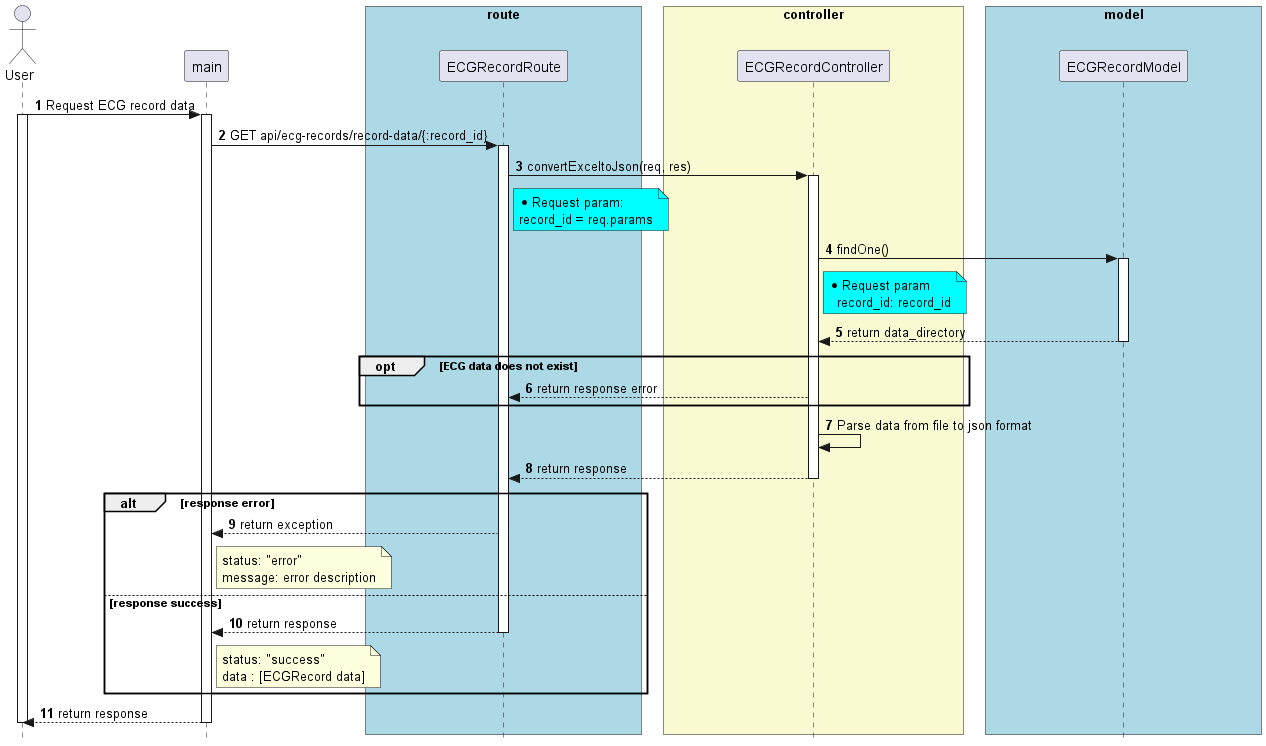
\includegraphics[width=16cm,height=9cm]{Images/server/sequence/server/convertExceltoJson.png}
  \caption[Sơ đồ tuần tự ]{\bfseries \fontsize{12pt}{0pt}
  \selectfont Sơ đồ tuần }
  \label{hinh21} %đặt tên cho ảnh
\end{figure}


\begin{figure}[H]
  \centering
  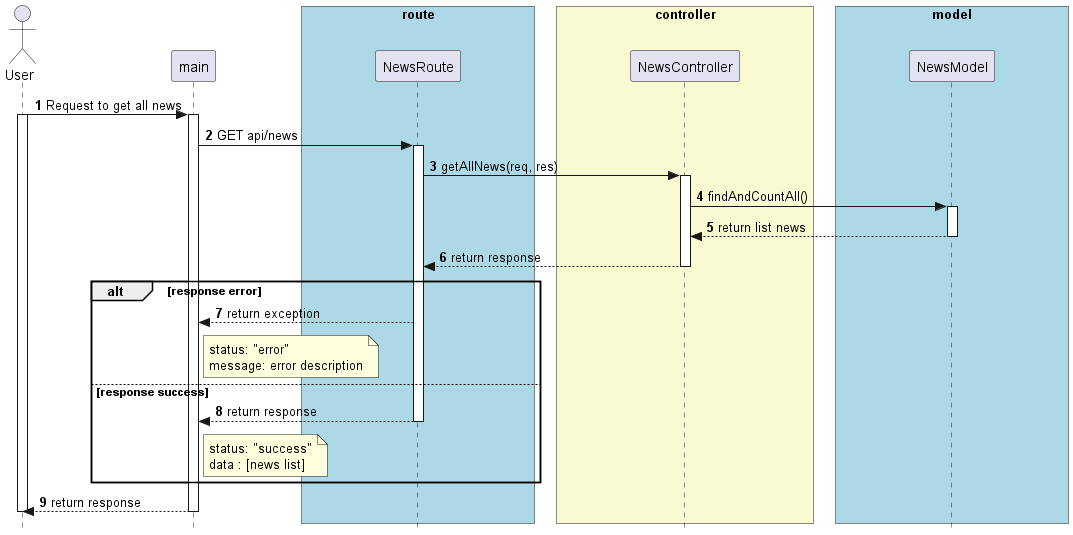
\includegraphics[width=16cm,height=9cm]{Images/server/sequence/server/getAllNews.png}
  \caption[Sơ đồ tuần tự ]{\bfseries \fontsize{12pt}{0pt}
  \selectfont Sơ đồ tuần }
  \label{hinh21} %đặt tên cho ảnh
\end{figure}

\begin{figure}[H]
  \centering
  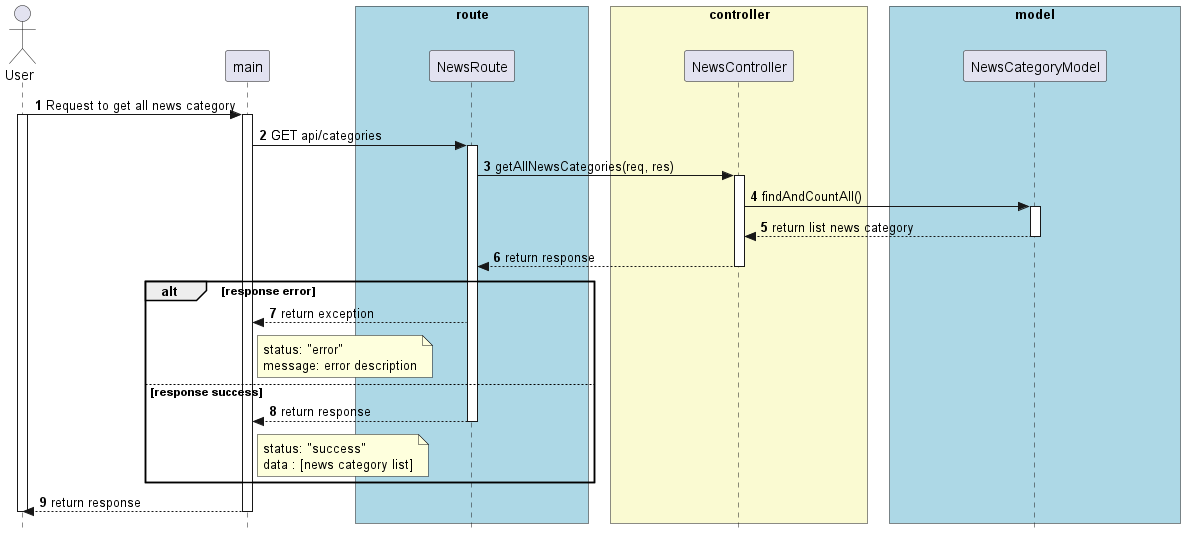
\includegraphics[width=16cm,height=9cm]{Images/server/sequence/server/getAllNewsCategories.png}
  \caption[Sơ đồ tuần tự ]{\bfseries \fontsize{12pt}{0pt}
  \selectfont Sơ đồ tuần }
  \label{hinh21} %đặt tên cho ảnh
\end{figure}


\begin{figure}[H]
  \centering
  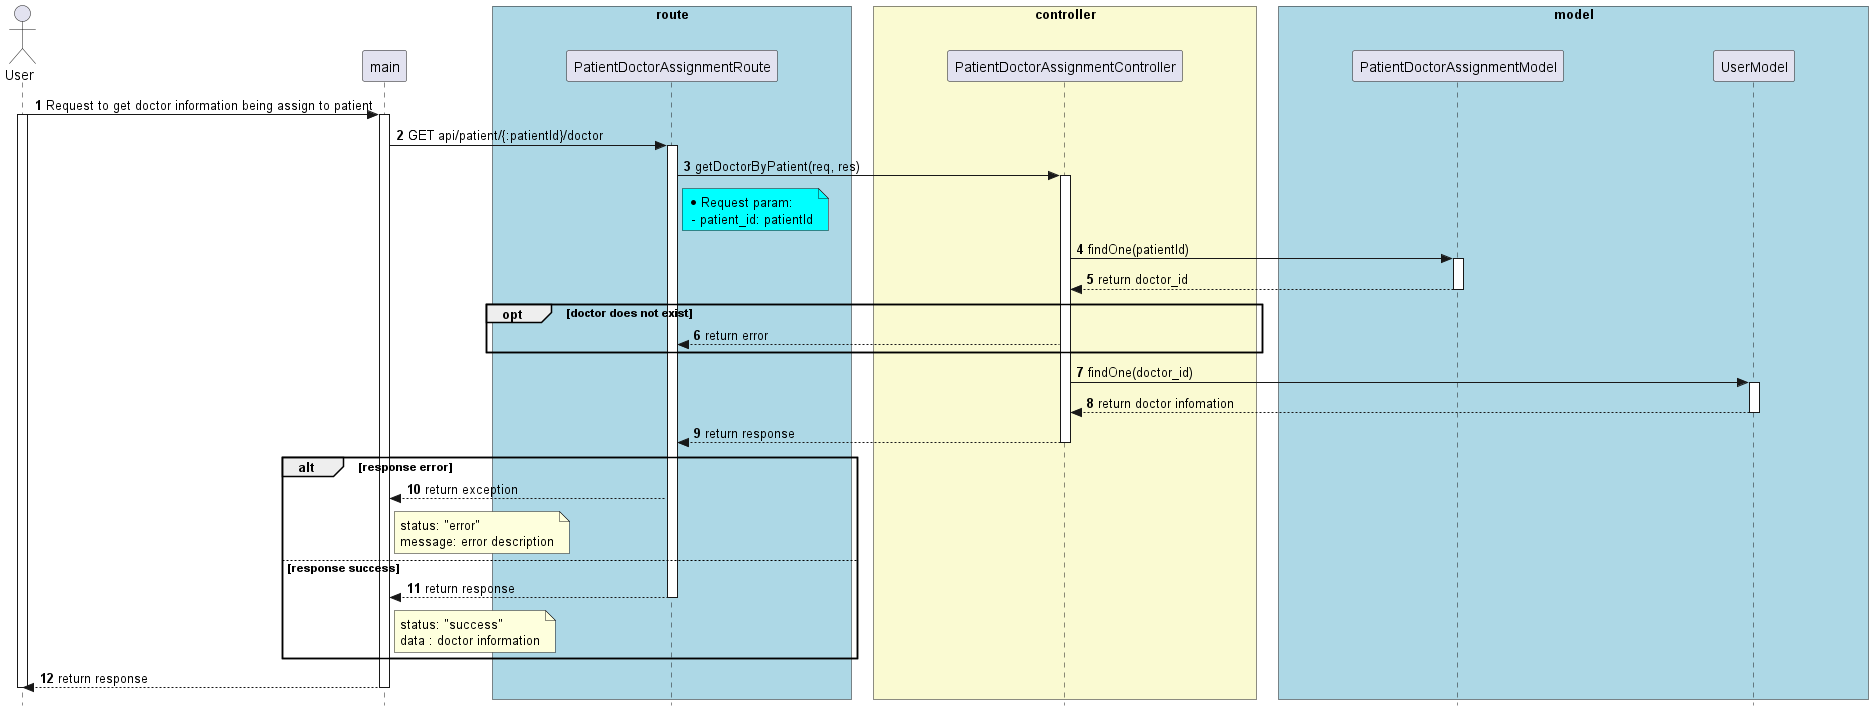
\includegraphics[width=16cm,height=9cm]{Images/server/sequence/server/getDoctorByPatient.png}
  \caption[Sơ đồ tuần tự ]{\bfseries \fontsize{12pt}{0pt}
  \selectfont Sơ đồ tuần }
  \label{hinh21} %đặt tên cho ảnh
\end{figure}


\begin{figure}[H]
  \centering
  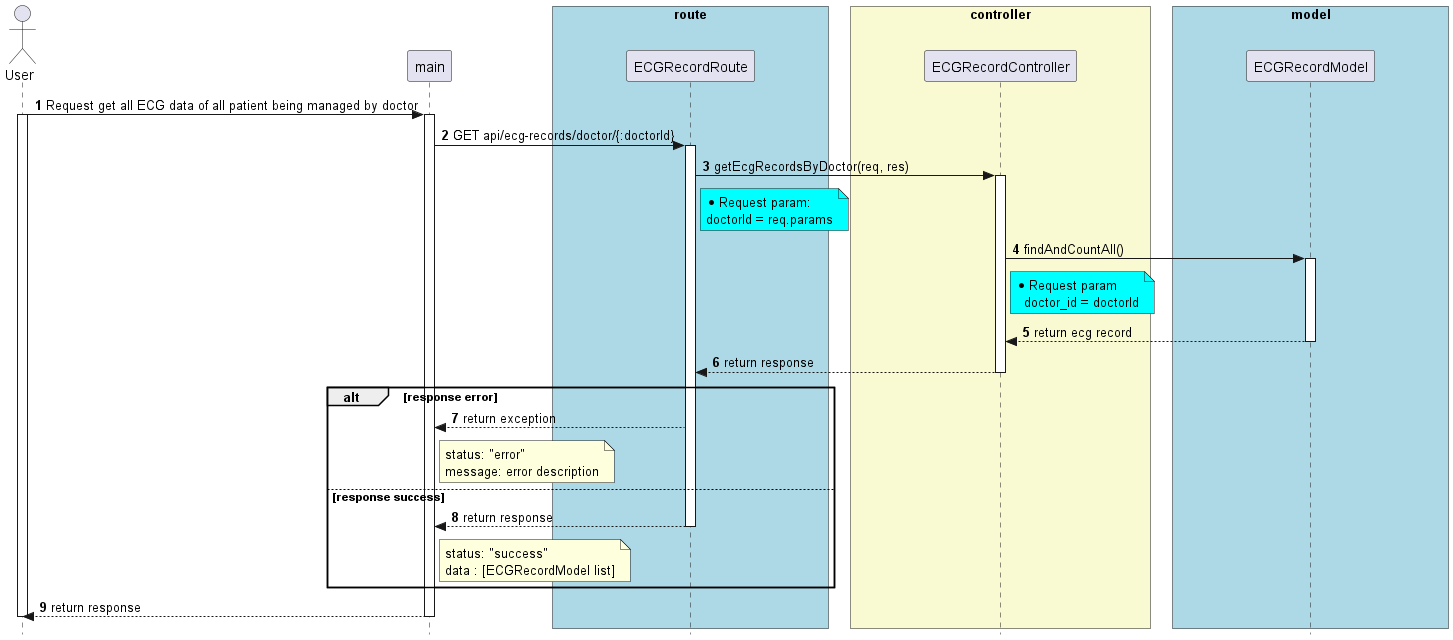
\includegraphics[width=16cm,height=9cm]{Images/server/sequence/server/getEcgRecordsByDoctor.png}
  \caption[Sơ đồ tuần tự ]{\bfseries \fontsize{12pt}{0pt}
  \selectfont Sơ đồ tuần }
  \label{hinh21} %đặt tên cho ảnh
\end{figure}


\begin{figure}[H]
  \centering
  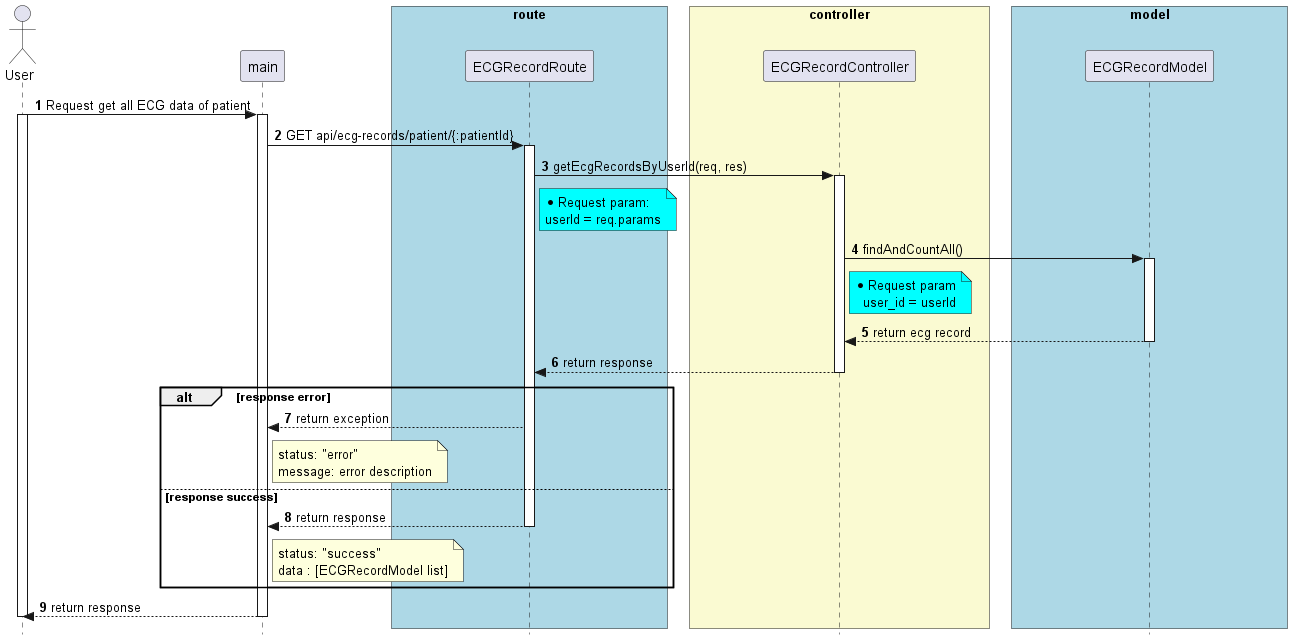
\includegraphics[width=16cm,height=9cm]{Images/server/sequence/server/getEcgRecordsByUserId.png}
  \caption[Sơ đồ tuần tự ]{\bfseries \fontsize{12pt}{0pt}
  \selectfont Sơ đồ tuần }
  \label{hinh21} %đặt tên cho ảnh
\end{figure}


\begin{figure}[H]
  \centering
  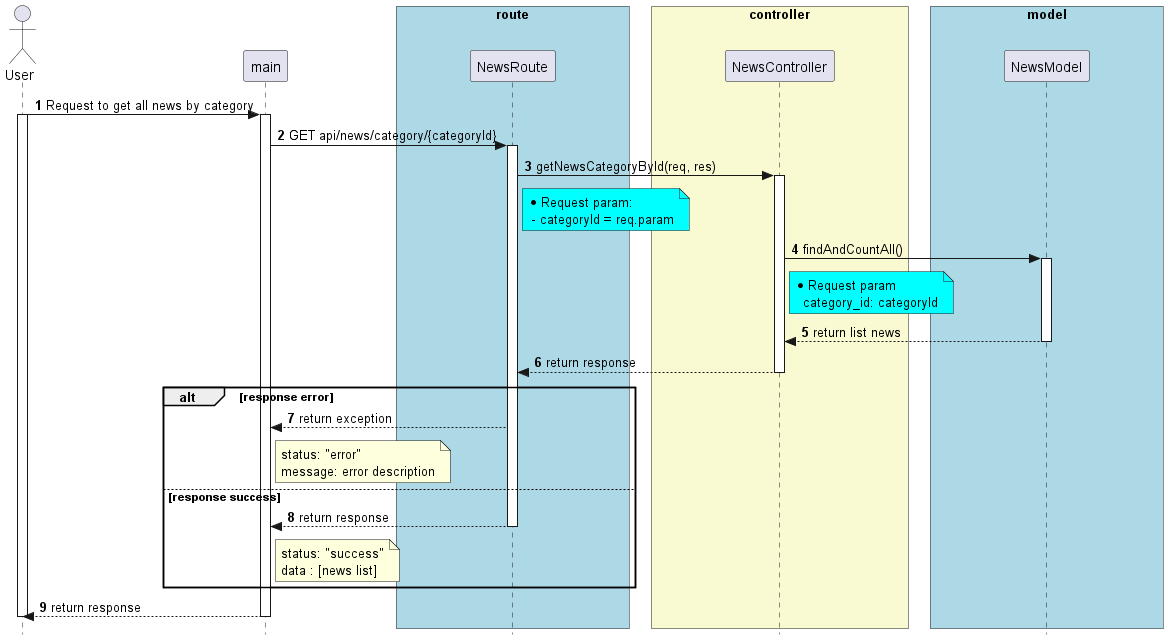
\includegraphics[width=16cm,height=9cm]{Images/server/sequence/server/getNewsByCategory.png}
  \caption[Sơ đồ tuần tự ]{\bfseries \fontsize{12pt}{0pt}
  \selectfont Sơ đồ tuần }
  \label{hinh21} %đặt tên cho ảnh
\end{figure}


\begin{figure}[H]
  \centering
  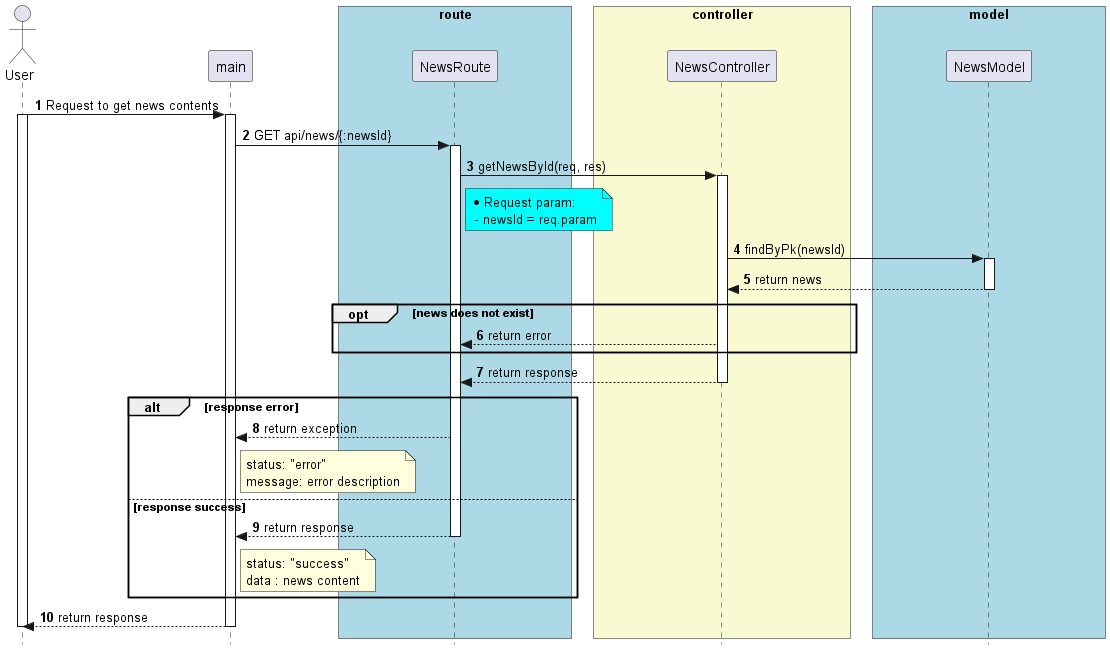
\includegraphics[width=16cm,height=9cm]{Images/server/sequence/server/getNewsById.png}
  \caption[Sơ đồ tuần tự ]{\bfseries \fontsize{12pt}{0pt}
  \selectfont Sơ đồ tuần }
  \label{hinh21} %đặt tên cho ảnh
\end{figure}


\begin{figure}[H]
  \centering
  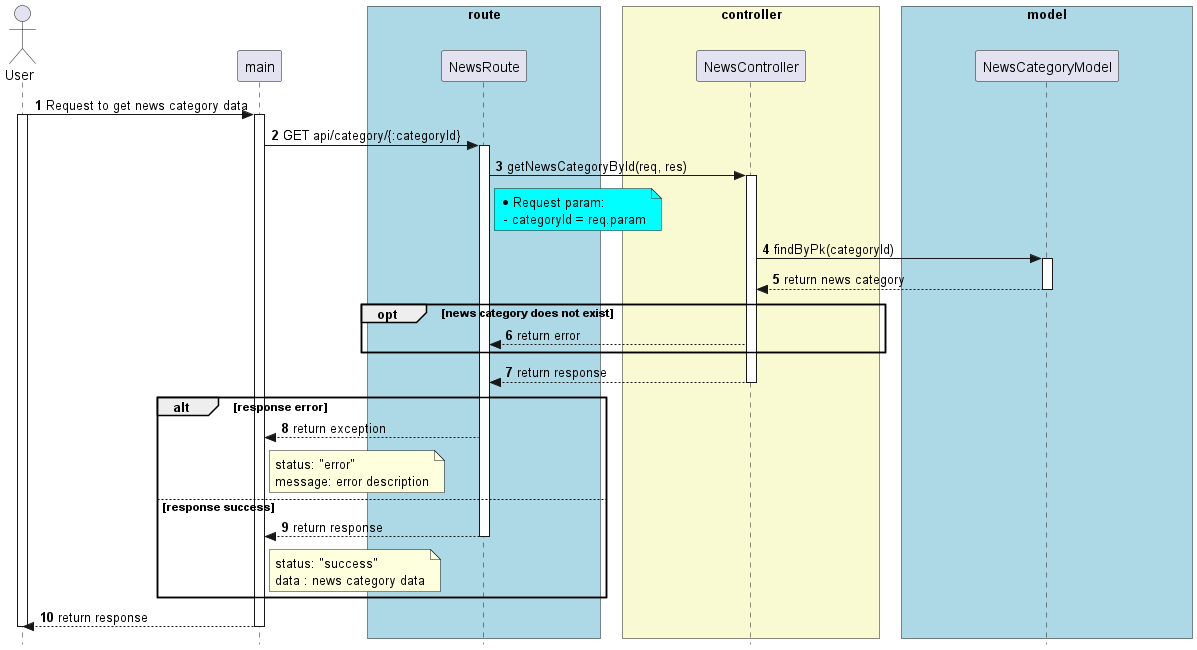
\includegraphics[width=16cm,height=9cm]{Images/server/sequence/server/getNewsCategoryById.png}
  \caption[Sơ đồ tuần tự ]{\bfseries \fontsize{12pt}{0pt}
  \selectfont Sơ đồ tuần }
  \label{hinh21} %đặt tên cho ảnh
\end{figure}

\begin{figure}[H]
  \centering
  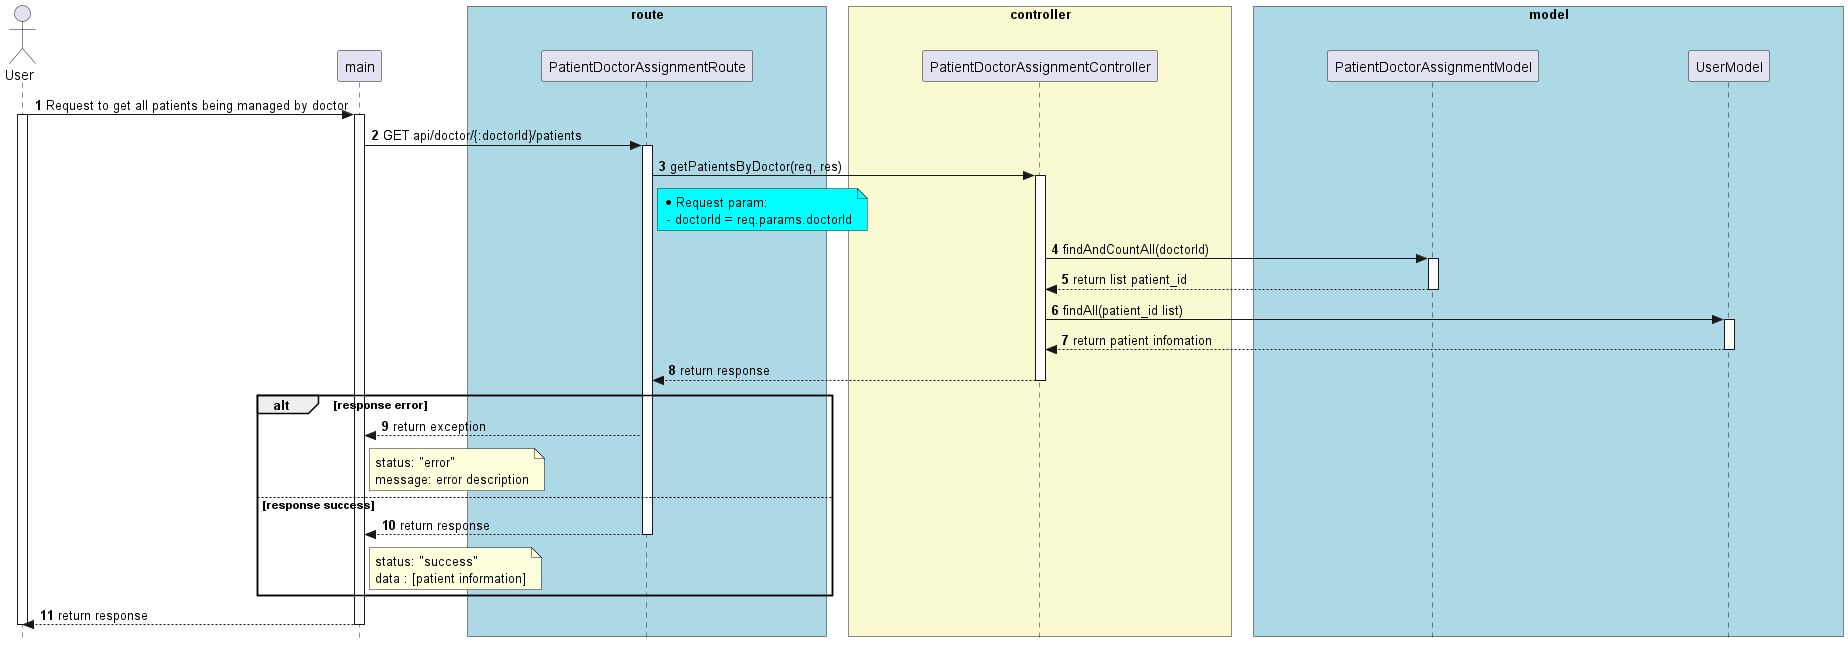
\includegraphics[width=16cm,height=9cm]{Images/server/sequence/server/getPatientsByDoctor.png}
  \caption[Sơ đồ tuần tự ]{\bfseries \fontsize{12pt}{0pt}
  \selectfont Sơ đồ tuần }
  \label{hinh21} %đặt tên cho ảnh
\end{figure}

\begin{figure}[H]
  \centering
  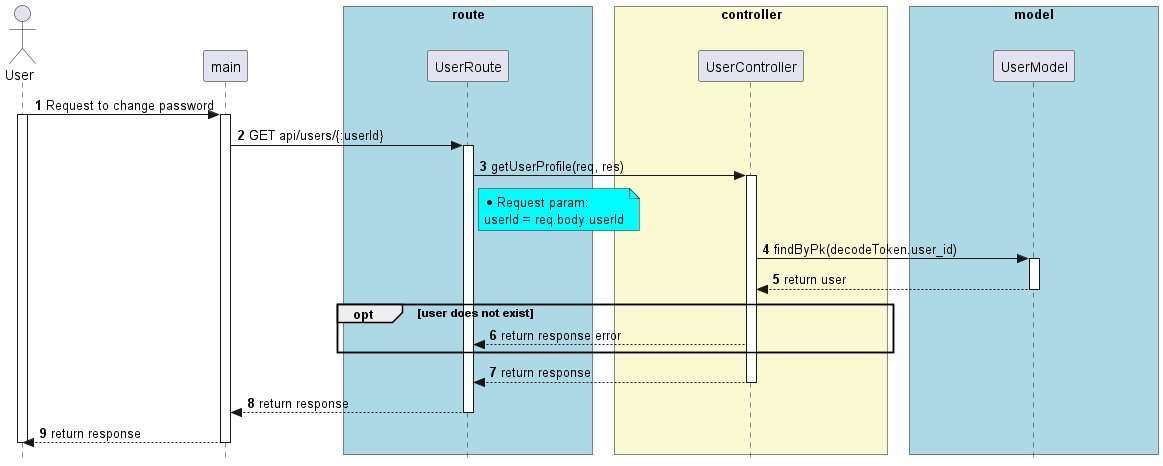
\includegraphics[width=16cm,height=9cm]{Images/server/sequence/server/getUserById.png}
  \caption[Sơ đồ tuần tự ]{\bfseries \fontsize{12pt}{0pt}
  \selectfont Sơ đồ tuần }
  \label{hinh21} %đặt tên cho ảnh
\end{figure}

\begin{figure}[H]
  \centering
  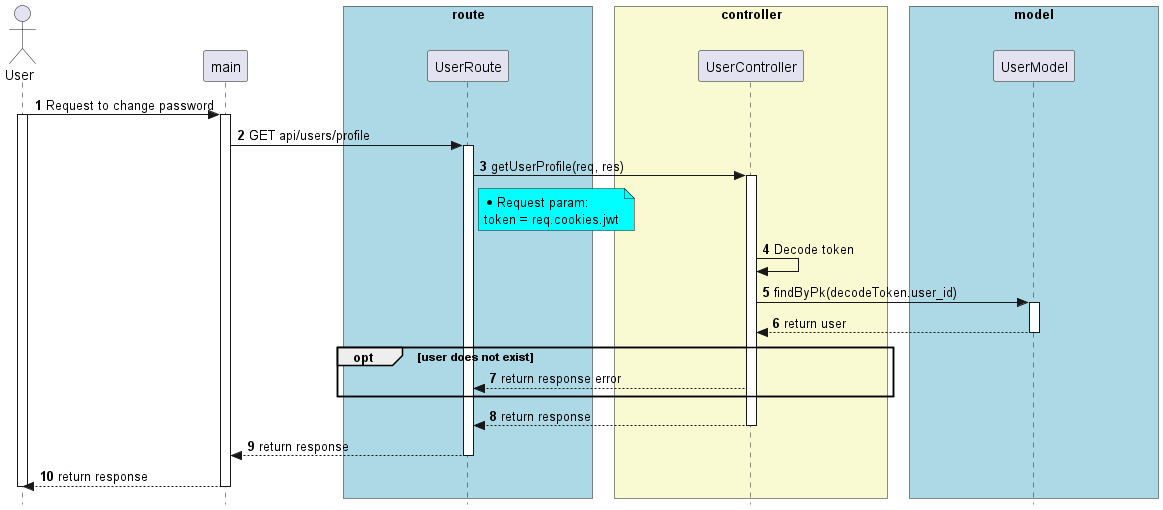
\includegraphics[width=16cm,height=9cm]{Images/server/sequence/server/getUserProfile.png}
  \caption[Sơ đồ tuần tự ]{\bfseries \fontsize{12pt}{0pt}
  \selectfont Sơ đồ tuần }
  \label{hinh21} %đặt tên cho ảnh
\end{figure}

\begin{figure}[H]
  \centering
  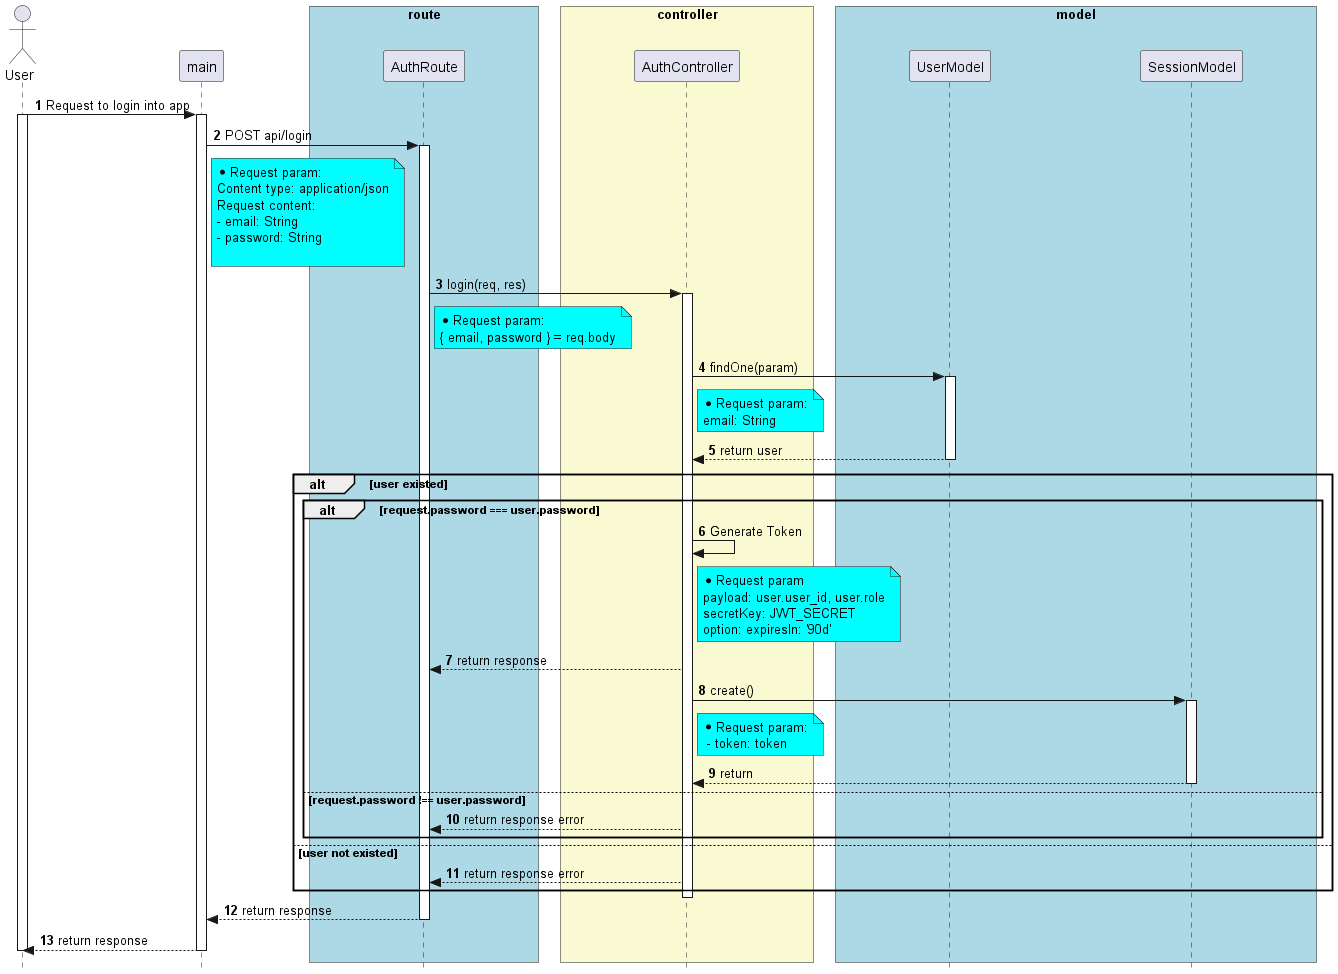
\includegraphics[width=16cm,height=9cm]{Images/server/sequence/server/login.png}
  \caption[Sơ đồ tuần tự ]{\bfseries \fontsize{12pt}{0pt}
  \selectfont Sơ đồ tuần }
  \label{hinh21} %đặt tên cho ảnh
\end{figure}

\begin{figure}[H]
  \centering
  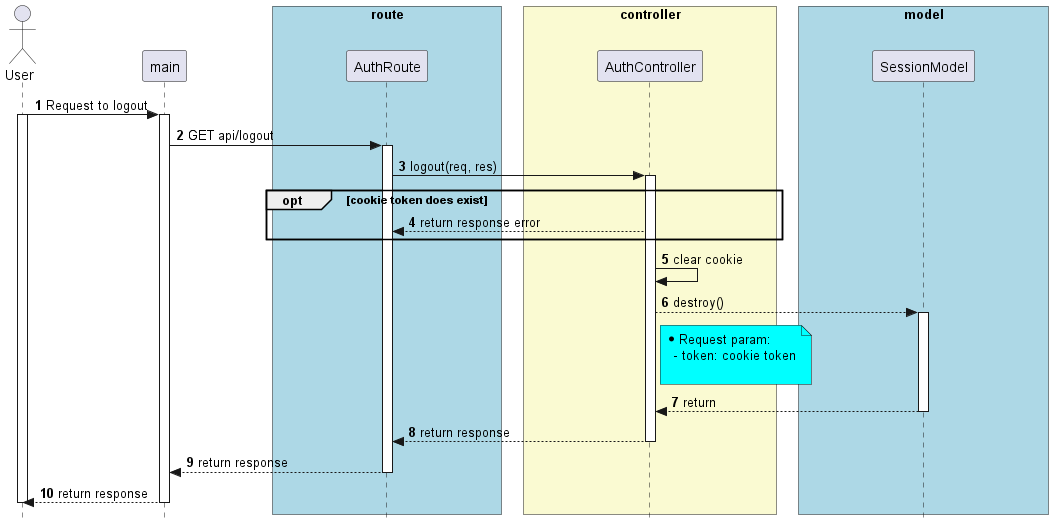
\includegraphics[width=16cm,height=9cm]{Images/server/sequence/server/logout.png}
  \caption[Sơ đồ tuần tự ]{\bfseries \fontsize{12pt}{0pt}
  \selectfont Sơ đồ tuần }
  \label{hinh21} %đặt tên cho ảnh
\end{figure}


\begin{figure}[H]
  \centering
  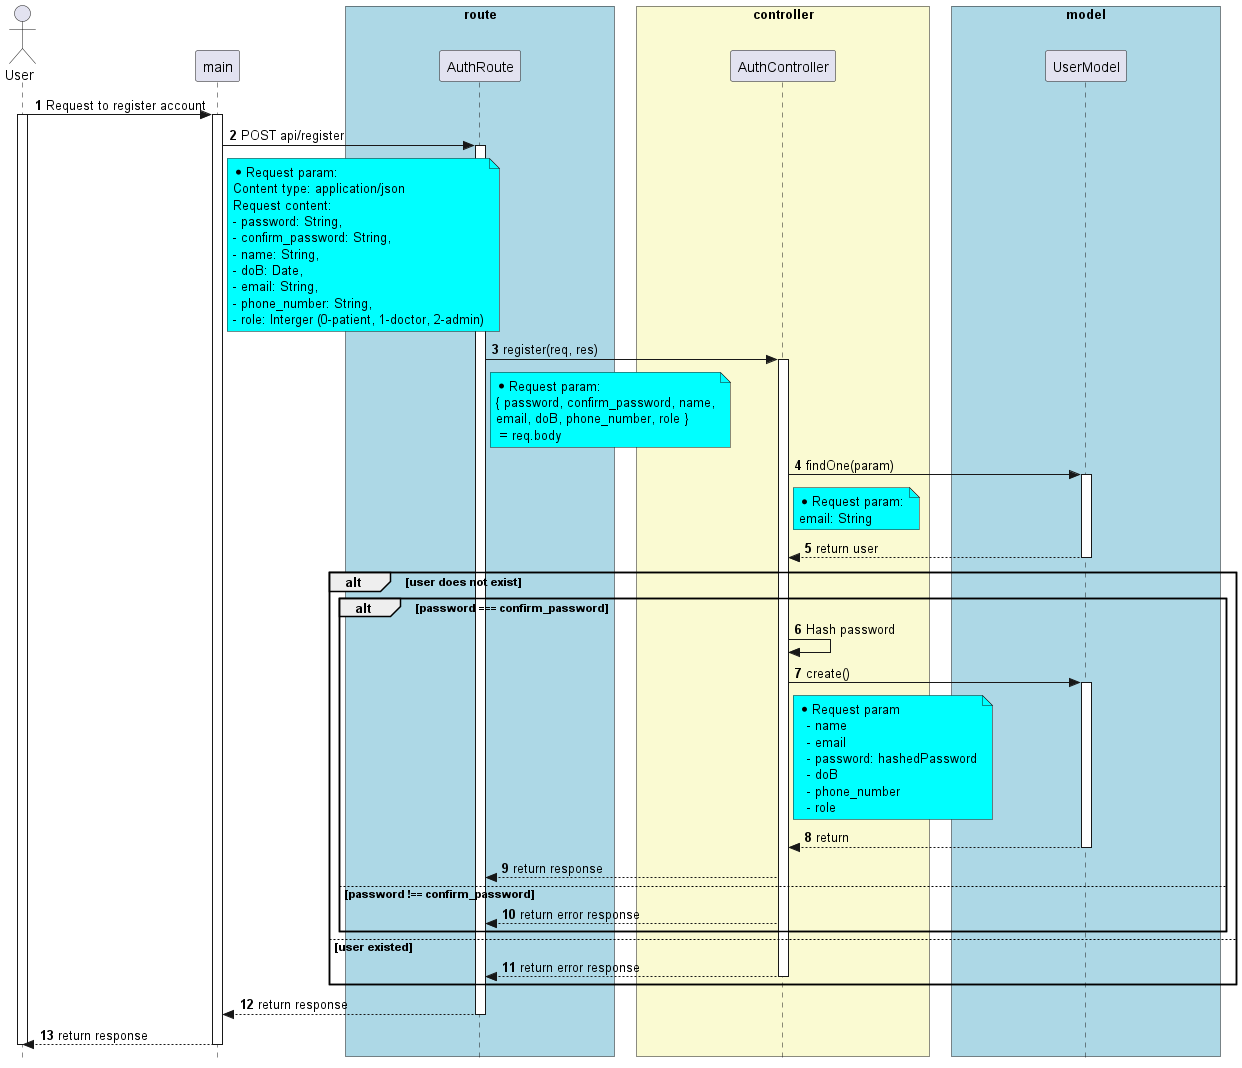
\includegraphics[width=16cm,height=9cm]{Images/server/sequence/server/register.png}
  \caption[Sơ đồ tuần tự ]{\bfseries \fontsize{12pt}{0pt}
  \selectfont Sơ đồ tuần }
  \label{hinh21} %đặt tên cho ảnh
\end{figure}

\begin{figure}[H]
  \centering
  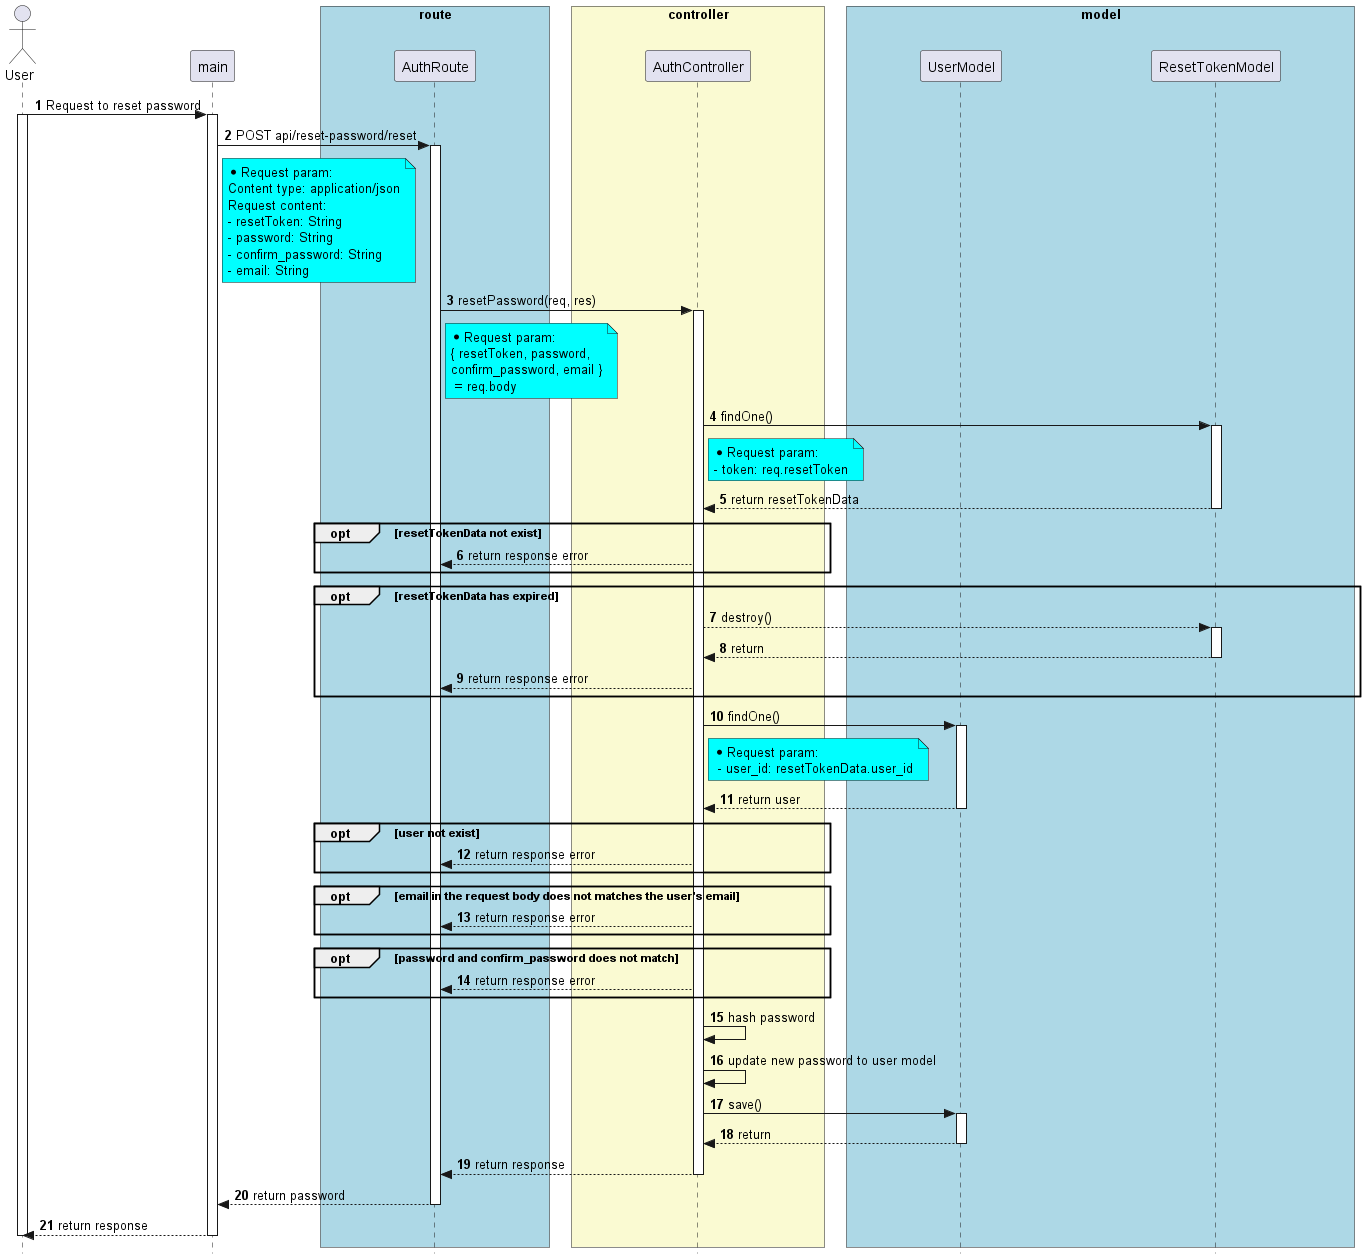
\includegraphics[width=16cm,height=9cm]{Images/server/sequence/server/resetPassword.png}
  \caption[Sơ đồ tuần tự ]{\bfseries \fontsize{12pt}{0pt}
  \selectfont Sơ đồ tuần }
  \label{hinh21} %đặt tên cho ảnh
\end{figure}

\begin{figure}[H]
  \centering
  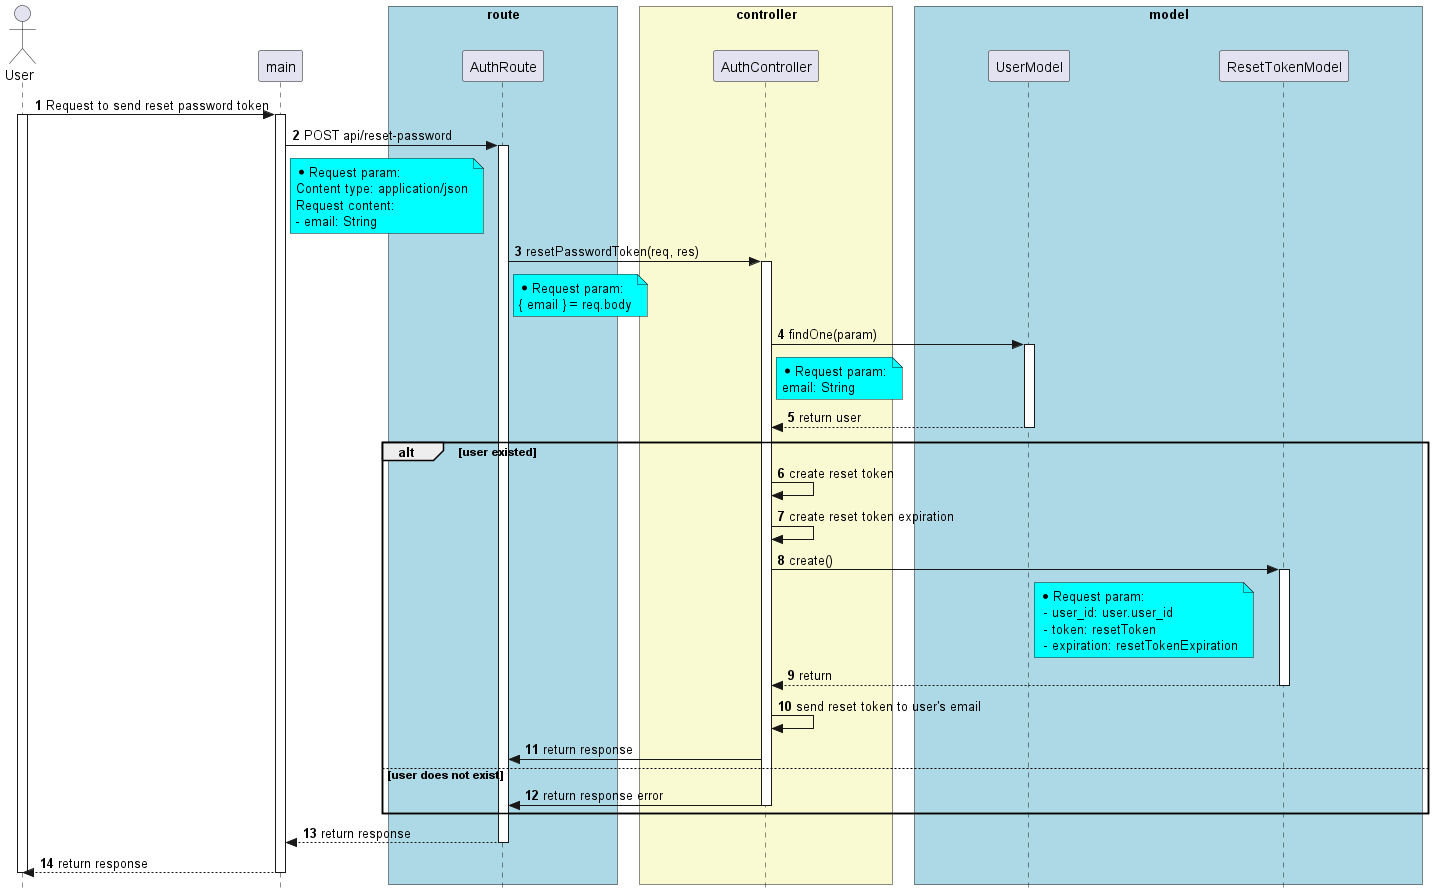
\includegraphics[width=16cm,height=9cm]{Images/server/sequence/server/resetPasswordToken.png}
  \caption[Sơ đồ tuần tự ]{\bfseries \fontsize{12pt}{0pt}
  \selectfont Sơ đồ tuần }
  \label{hinh21} %đặt tên cho ảnh
\end{figure}

\begin{figure}[H]
  \centering
  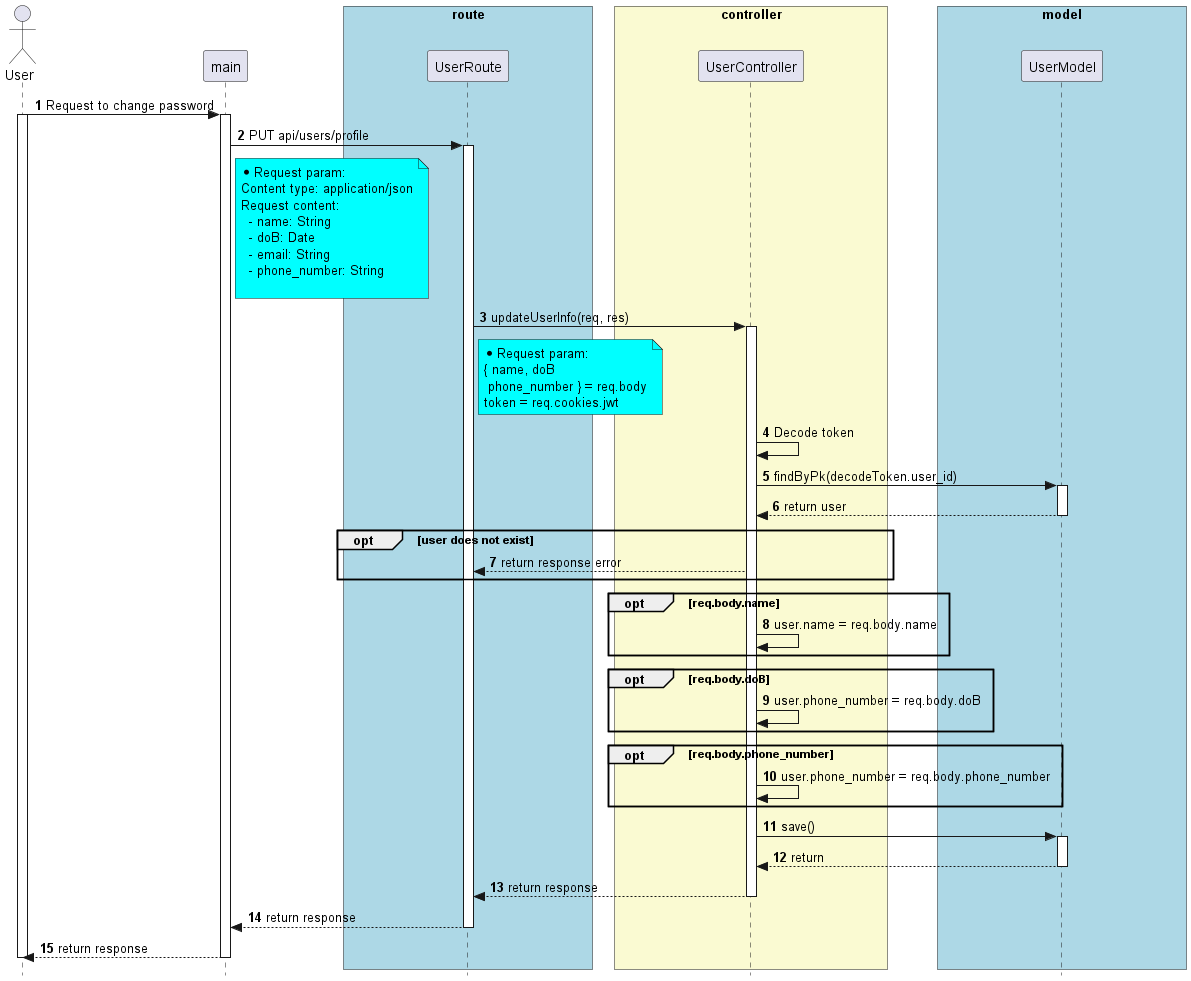
\includegraphics[width=16cm,height=9cm]{Images/server/sequence/server/updateUserInfo.png}
  \caption[Sơ đồ tuần tự ]{\bfseries \fontsize{12pt}{0pt}
  \selectfont Sơ đồ tuần }
  \label{hinh21} %đặt tên cho ảnh
\end{figure}



\begin{figure}[H]
  \centering
  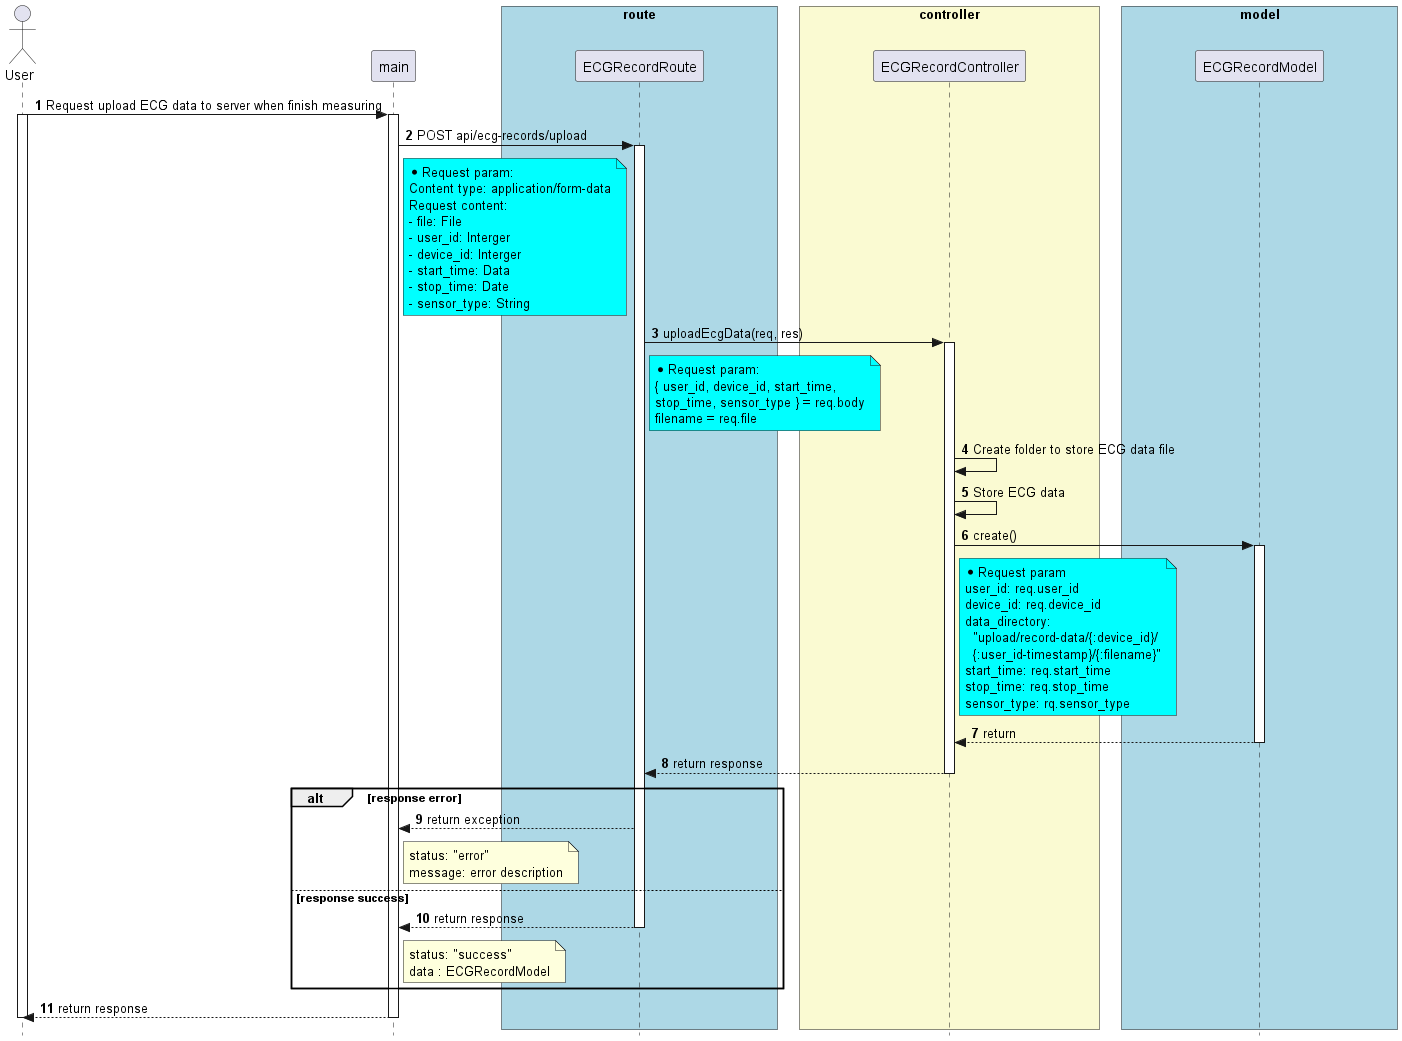
\includegraphics[width=16cm,height=9cm]{Images/server/sequence/server/uploadEcgData.png}
  \caption[Sơ đồ tuần tự ]{\bfseries \fontsize{12pt}{0pt}
  \selectfont Sơ đồ tuần }
  \label{hinh21} %đặt tên cho ảnh
\end{figure}


\begin{figure}[H]
  \centering
  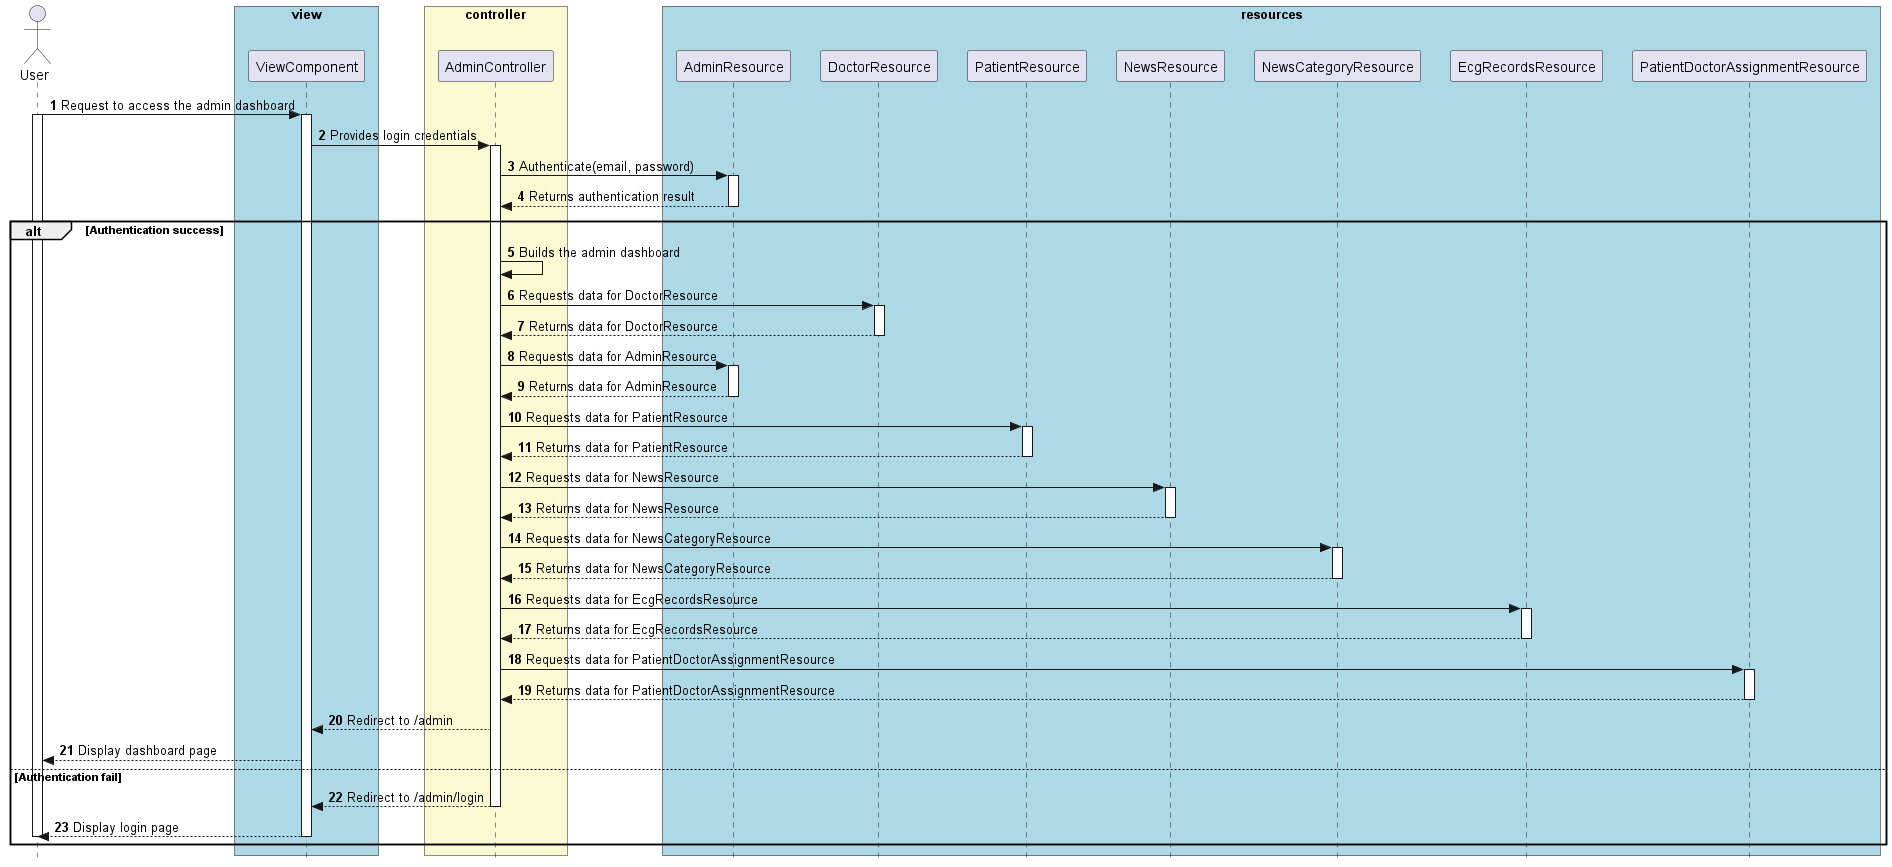
\includegraphics[width=16cm,height=9cm]{Images/server/sequence/web/seq_auth.png}
  \caption[Sơ đồ tuần tự ]{\bfseries \fontsize{12pt}{0pt}
  \selectfont Sơ đồ tuần }
  \label{hinh21} %đặt tên cho ảnh
\end{figure}

\begin{figure}[H]
  \centering
  \includegraphics[width=16cm,height=9cm]{Images/server/sequence/web/seq_crud.png}
  \caption[Sơ đồ tuần tự ]{\bfseries \fontsize{12pt}{0pt}
  \selectfont Sơ đồ tuần }
  \label{hinh21} %đặt tên cho ảnh
\end{figure}


\newpage
\section*{CHƯƠNG 3. TRIỂN KHAI VÀ KIỂM THỬ}
\setcounter{section}{3}
\setcounter{subsection}{0} %LƯU Ý MỖI LẦN THÊM CHƯƠNG MỚI CẦN THÊM CÂU NÀY ĐỂ RESET THỨ TỰ CỦA SUBSECTON VỀ 1
\setcounter{table}{0} % LƯU Ý SAU MỖI LẦN GỌI BẢNG HAY HÌNH ẢNH PHẢI THÊM CÂU NÀY ĐỂ RESET THỨ TỰ
\setcounter{figure}{0} %% LƯU Ý SAU MỖI LẦN GỌI BẢNG HAY HÌNH ẢNH PHẢI THÊM CÂU NÀY ĐỂ RESET THỨ TỰ
\addcontentsline{toc}{section}{\numberline{}CHƯƠNG 3. TRIỂN KHAI VÀ KIỂM THỬ}

\section*{CHƯƠNG 4. THÍ NGHIỆM VÀ KẾT QUẢ}
\setcounter{section}{4}
\setcounter{equation}{0}

\setcounter{subsection}{0} %LƯU Ý MỖI LẦN THÊM CHƯƠNG MỚI CẦN THÊM CÂU NÀY ĐỂ RESET THỨ TỰ CỦA SUBSECTON VỀ 1
\setcounter{table}{0} % LƯU Ý SAU MỖI LẦN GỌI BẢNG HAY HÌNH ẢNH PHẢI THÊM CÂU NÀY ĐỂ RESET THỨ TỰ
\setcounter{figure}{0} %% LƯU Ý SAU MỖI LẦN GỌI BẢNG HAY HÌNH ẢNH PHẢI THÊM CÂU NÀY ĐỂ RESET THỨ TỰ
\addcontentsline{toc}{section}{\numberline{}CHƯƠNG 4. THÍ NGHIỆM VÀ KẾT QUẢ}
\subsection{ABF}
\lipsum
% \begin{figure}[H]
%      \centering
%      \includegraphics[width=16cm,height=4.39cm]{Images/ly-thuyet-bai-17-he-thong-thong-tin-va-vien-thong.png}
%      \caption[Sơ đồ khối của hệ thống]{\bfseries \fontsize{12pt}{0pt}\selectfont Sơ đồ khối của hệ thống}
%      \label{hinh41} %đặt tên cho ảnh
% \end{figure}
% Hình \ref{hinh41} là ví dụ về cách chèn ảnh. Lưu ý chú thích của hình vẽ được đặt ngay dưới hình vẽ. Tất cả các hình vẽ 
% phải được đề cập đến trong phần nội  dung vÀ phải được phân tích và bình luận như đang làm

% \begin{figure}[H]
%      \centering
%      \includegraphics[width=16cm,height=4.39cm]{Images/ly-thuyet-bai-17-he-thong-thong-tin-va-vien-thong.png}
%      \caption[Sơ đồ khối của hệ thống]{\bfseries \fontsize{12pt}{0pt}\selectfont Sơ đồ khối của hệ thống}
%      \label{hinh42} %đặt tên cho ảnh
% \end{figure}
Hình \ref{hinh42} là ví dụ về cách chèn ảnh. Lưu ý chú thích của hình vẽ được đặt ngay dưới hình vẽ. Tất cả các hình vẽ 
phải được đề cập đến trong phần nội  dung vÀ phải được phân tích và bình luận như đang làm

\begin{table}[H]
     \centering
     \caption{\bfseries \fontsize{12pt}{0pt}\selectfont Kết quả thí nghiệm}
     \begin{tabularx}{0.85\textwidth}{
     | >{\centering\arraybackslash}s
     | >{\centering\arraybackslash}X
     | >{\centering\arraybackslash}a
     | >{\centering\arraybackslash}s|
     }
     \hline
     \bfseries Lần thí nghiệm     &\bfseries Điện áp đo được\hspace{1cm}(mV)   &\bfseries Điện áp tham chiếu\hspace{0pt}(mV)    &\bfseries Sai lệch\hspace{0pt}  (\%)\\ \hline
     1   &    &    &\\ \hline
     2   &    &    &\\ \hline
     3   &    &    &\\ \hline
     ... &    &    &\\ \hline
     \end{tabularx}
     \label{bang41}
\end{table}
Bảng \ref{bang41} là ví dụ về cách tạo bảng. Lưu ý chú thích của bảng được đặt ở trước bảng. Tất cả các bảng biểu được đề cập
đến trong phần nội dung và phải được phân tích và bình luận như đang làm

\begin{equation}
     F(x) = \int^a_b \frac{1}{3}x^3
     \label{pt31}
\end{equation}
 Phương trình \ref{pt31} là ví dụ về phương trình tích phân


\cleardoublepage
\section*{KẾT LUẬN}
\phantomsection\addcontentsline{toc}{section}{\numberline{} KẾT LUẬN}
\subsection*{Kết luận chung}
\addcontentsline{toc}{section}{\numberline{} Kết luận chung}
Kết luận chung cho các chương trong đồ án. Mục này cần nhấn mạnh những vấn đề đã giải
quyết và vấn đề chưa giải quyết để đưa ra các đánh giá về mức độ hoàn thành cô việc. Đánh 
giá này thường so sánh kết quả thu được với mục tiêu đề ra ban đầu 

\subsection*{Hướng phát triển}
\phantomsection\addcontentsline{toc}{section}{\numberline{} Hướng phát triển}
(Nếu có) \cite{nhu2019effects}

\subsection*{Kiến nghị và đề xuất}
\phantomsection\addcontentsline{toc}{section}{\numberline{} Kiến nghị và đề xuất}
(nếu có)

\cleardoublepage


\phantomsection\addcontentsline{toc}{section}{\numberline{} TÀI LIỆU THAM KHẢO}
\bibliographystyle{IEEEtran}
\bibliography{TaiLieuThamKhao}

\cleardoublepage
\section*{PHỤ LỤC}
\phantomsection\addcontentsline{toc}{section}{\numberline{} PHỤ LỤC}
\texttt{\fontsize{10pt}{0pt}\selectfont Mã nguồn chương trình nếu có được đưa và đây sử dụng font 
Courier New, cỡ 10pt.}

\clearpage
\newpage \pagestyle{empty}
\begin{center}
    \textbf{\fontsize{14pt}{0pt}\selectfont ĐÁNH GIÁ QUYỂN ĐỒ ÁN TỐT NGHIỆP}\\
    \vspace{10pt}
    \fontsize{14pt}{0pt}\selectfont (Dùng cho giản viên hướng dẫn) 
\end{center}
\vspace{14pt}
\fontsize{13pt}{20pt}\selectfont Tên giảng viên đánh giá:\\
\fontsize{13pt}{20pt}\selectfont Họ và tên Sinh Viên:
\hspace{5.5cm}
\fontsize{13pt}{20pt}\selectfont MSSV:\\
\fontsize{13pt}{20pt}\selectfont Tên đồ án:\\
\fontsize{13pt}{20pt}\selectfont \\
\textbf{\fontsize{13pt}{20pt}\selectfont Chọn các mức điểm phù hợp cho sinh viên trình bày theo các tiêu chí dưới đây:}\\
\fontsize{13pt}{20pt}\selectfont Rất kém (1); Kém (2); Đạt (3); Giỏi (4); Xuất sắc (5)
\begin{table}[H]
    \fontsize{11}{11}\selectfont
    \begin{tabular}{|M{1cm}|M{11cm}|M{0.3cm}|M{0.3cm}|M{0.3cm}|M{0.3cm}|M{0.3cm}|}
    \hline
    \rowcolor[rgb]{0.52,0.96,1}
    \multicolumn{7}{|p{1.01\linewidth}|}{\textbf{Có sự kết hợp giữa lý thuyết va thực hành (20)}} \\
    \hline
    1 &  \raggedright Nêu rõ tính cấp thiết và quan trọng của đề tài, các cấn đề và các giả thuyết (bao gồm mục đíc và tính phù hợp) cũng như phạm vi ứng dụng của đồ án  & 1 & 2 & 3 & 4 & 5\\
    \hline
    2 & \raggedright Cập nhật kết quả nghiên cứu gần đây nhất (trong nước/quốc tế) & 1 & 2 & 3 & 4 & 5\\
    \hline
    3 & \raggedright Nêu rõ và chi tiết phương pháp nghiên cứu/giải quyết vấn đề & 1 & 2 & 3 & 4 & 5\\
    \hline
    4 & \raggedright Có kết quả mô phỏng/thực nghiệm và trình bày rõ ràng kết quả đo được & 1 & 2 & 3 & 4 & 5\\
    \hline
    
    \rowcolor[rgb]{0.52,0.96,1}
    \multicolumn{7}{|p{1.01\linewidth}|}{\textbf{Có khả năng phân tích và đánh giá kết quả (15)}} \\
    \hline
    5 &  \raggedright Kế hoạch làm việc rõ ràng bao gồm mục tiêu và phương pháp thực hiện dựa trên kết quả nghiên cứu lý thuyết một cách có hệ thống  & 1 & 2 & 3 & 4 & 5\\
    \hline
    6 & \raggedright Kết quả được trình bày một cách logic và dễ hiểu, tất cả kết quả đều được phân tích và đánh giá thỏa đáng. & 1 & 2 & 3 & 4 & 5\\
    \hline
    7 & \raggedright Trong phần kết luận, tác giả chỉ rõ sự khác biệt (nếu có) giữa kết quả đạt được và mục tiêu ban đầu đề ra đồng thời cung cấp lập luận để đề xuất hướng giải quyết có thể thực hiện trong tương lai. & 1 & 2 & 3 & 4 & 5\\
    \hline
    
    \rowcolor[rgb]{0.52,0.96,1}
    \multicolumn{7}{|p{1.01\linewidth}|}{\textbf{Kỹ năng viết quyển đồ án (10)}} \\
    \hline
    8 &  \raggedright Đồ án trình bày đúng mẫu quy định với cấu trúc các chương logic và đẹp mắt (bảng biểu, hình ảnh rõ ràng, có tiêu đề, được đánh số thứ tự và được giải thích hay đề cập đến trong đồ án, có căn lề, dấu cách sau dấu chấm, dấu phẩy v.v), có mở đầu chương và kết luận chương, có liệt kê tài liệu tham khảo và có trích dẫn đúng quy địnhg  & 1 & 2 & 3 & 4 & 5\\
    \hline
    9 & \raggedright Kỹ năng viết xuất sắc (cấu trúc câu chuẩn, văn phong khoa học, lập luận logic và có cơ sở, từ vựng sử dụng phù hợp v.v.). & 1 & 2 & 3 & 4 & 5\\
    \hline
    
    \rowcolor[rgb]{0.52,0.96,1}
    \multicolumn{7}{|p{1.01\linewidth}|}{\textbf{Thành tựu nghiên cứu khoa học (5) (chọn 1 trong 3 trường hợp)}} \\
    \hline
    10a &  \raggedright Có bài báo khoa học được đăng hoặc chấp nhận đăng/đạt giải SVNC khoa học giải 3 cấp  Viện trở lên/các giải thưởng khoa học (quốc tế/trong nước) từ giải 3 trở lên/ Có đăng ký bằng phát minh sáng chế  & 1 & 2 & 3 & 4 & 5\\
    \hline
    10b & \raggedright Được báo cáo tại hội đồng cấp Viện trong hội nghị sinh viên nghiên cứu khoa học nhưng không đạt giải từ giải 3 trở lên/Đạt giải khuyến khích trong các kỳ thi quốc gia và quốc tế khác về chuyên ngành như TI contest.). & 1 & 2 & 3 & 4 & 5\\
    \hline
    10c & \raggedright Không có thành tích về nghiên cứu khoa học & 1 & 2 & 3 & 4 & 5\\
    \hline
    \rowcolor[rgb]{0.52,0.96,1}
    \multicolumn{2}{|p{0.776\linewidth}|}{\textbf{Điểm tổng}} & \multicolumn{5}{|p{0.205\linewidth}|}{\textbf{\hspace{2cm}/50}} \\
    \hline
    \rowcolor[rgb]{0.52,0.96,1}
    \multicolumn{2}{|p{0.776\linewidth}|}{\textbf{Điểm tổng quy đổi về thang 10}}&\multicolumn{5}{|p{0.205\linewidth}|}{} \\
    \hline
    \end{tabular}
    \label{mul_table}
\end{table}
\raggedright\textbf{\itshape\fontsize{13pt}{20pt}\selectfont Nhận xét khác} \fontsize{13pt}{20pt}\selectfont (về thái độ và tinh thần làm việc của sinh viên)
\newline



\vspace{5cm}
\hspace{9cm}Hà Nội, ngày\hspace{0.5cm}tháng\hspace{0.5cm}năm

\hspace{10cm}\textbf{Người nhận xét}
\vspace{2cm}
\hspace{9.5cm} (Ký và ghi rõ họ tên)
\newpage
\begin{center}
    \textbf{\fontsize{14pt}{0pt}\selectfont ĐÁNH GIÁ QUYỂN ĐỒ ÁN TỐT NGHIỆP}\\
    \vspace{10pt}
    \fontsize{14pt}{0pt}\selectfont (Dùng cho cán bộ phản biện) 
\end{center}
\vspace{14pt}
\fontsize{13pt}{20pt}\selectfont Tên giảng viên đánh giá:\\
\fontsize{13pt}{20pt}\selectfont Họ và tên Sinh Viên:
\hspace{5.5cm}
\fontsize{13pt}{20pt}\selectfont MSSV:\\
\fontsize{13pt}{20pt}\selectfont Tên đồ án:\\

\vspace{0.8cm}

\textbf{\fontsize{13pt}{20pt}\selectfont Chọn các mức điểm phù hợp cho sinh viên trình bày theo các tiêu chí dưới đây:}\\
\fontsize{13pt}{20pt}\selectfont Rất kém (1); Kém (2); Đạt (3); Giỏi (4); Xuất sắc (5)
\begin{table}[H]
    \fontsize{11}{11}\selectfont
    \begin{tabular}{|M{1cm}|M{11cm}|M{0.3cm}|M{0.3cm}|M{0.3cm}|M{0.3cm}|M{0.3cm}|}
    \hline
    \rowcolor[rgb]{0.52,0.96,1}
    \multicolumn{7}{|p{1.01\linewidth}|}{\textbf{Có sự kết hợp giữa lý thuyết va thực hành (20)}} \\
    \hline
    1 &  \raggedright Nêu rõ tính cấp thiết và quan trọng của đề tài, các cấn đề và các giả thuyết (bao gồm mục đíc và tính phù hợp) cũng như phạm vi ứng dụng của đồ án  & 1 & 2 & 3 & 4 & 5\\
    \hline
    2 & \raggedright Cập nhật kết quả nghiên cứu gần đây nhất (trong nước/quốc tế) & 1 & 2 & 3 & 4 & 5\\
    \hline
    3 & \raggedright Nêu rõ và chi tiết phương pháp nghiên cứu/giải quyết vấn đề & 1 & 2 & 3 & 4 & 5\\
    \hline
    4 & \raggedright Có kết quả mô phỏng/thực nghiệm và trình bày rõ ràng kết quả đo được & 1 & 2 & 3 & 4 & 5\\
    \hline
    
    \rowcolor[rgb]{0.52,0.96,1}
    \multicolumn{7}{|p{1.01\linewidth}|}{\textbf{Có khả năng phân tích và đánh giá kết quả (15)}} \\
    \hline
    5 &  \raggedright Kế hoạch làm việc rõ ràng bao gồm mục tiêu và phương pháp thực hiện dựa trên kết quả nghiên cứu lý thuyết một cách có hệ thống  & 1 & 2 & 3 & 4 & 5\\
    \hline
    6 & \raggedright Kết quả được trình bày một cách logic và dễ hiểu, tất cả kết quả đều được phân tích và đánh giá thỏa đáng. & 1 & 2 & 3 & 4 & 5\\
    \hline
    7 & \raggedright Trong phần kết luận, tác giả chỉ rõ sự khác biệt (nếu có) giữa kết quả đạt được và mục tiêu ban đầu đề ra đồng thời cung cấp lập luận để đề xuất hướng giải quyết có thể thực hiện trong tương lai. & 1 & 2 & 3 & 4 & 5\\
    \hline
    
    \rowcolor[rgb]{0.52,0.96,1}
    \multicolumn{7}{|p{1.01\linewidth}|}{\textbf{Kỹ năng viết quyển đồ án (10)}} \\
    \hline
    8 &  \raggedright Đồ án trình bày đúng mẫu quy định với cấu trúc các chương logic và đẹp mắt (bảng biểu, hình ảnh rõ ràng, có tiêu đề, được đánh số thứ tự và được giải thích hay đề cập đến trong đồ án, có căn lề, dấu cách sau dấu chấm, dấu phẩy v.v), có mở đầu chương và kết luận chương, có liệt kê tài liệu tham khảo và có trích dẫn đúng quy địnhg  & 1 & 2 & 3 & 4 & 5\\
    \hline
    9 & \raggedright Kỹ năng viết xuất sắc (cấu trúc câu chuẩn, văn phong khoa học, lập luận logic và có cơ sở, từ vựng sử dụng phù hợp v.v.). & 1 & 2 & 3 & 4 & 5\\
    \hline
    
    \rowcolor[rgb]{0.52,0.96,1}
    \multicolumn{7}{|p{1.01\linewidth}|}{\textbf{Thành tựu nghiên cứu khoa học (5) (chọn 1 trong 3 trường hợp)}} \\
    \hline
    10a &  \raggedright Có bài báo khoa học được đăng hoặc chấp nhận đăng/đạt giải SVNC khoa học giải 3 cấp  Viện trở lên/các giải thưởng khoa học (quốc tế/trong nước) từ giải 3 trở lên/ Có đăng ký bằng phát minh sáng chế  & 1 & 2 & 3 & 4 & 5\\
    \hline
    10b & \raggedright Được báo cáo tại hội đồng cấp Viện trong hội nghị sinh viên nghiên cứu khoa học nhưng không đạt giải từ giải 3 trở lên/Đạt giải khuyến khích trong các kỳ thi quốc gia và quốc tế khác về chuyên ngành như TI contest.). & 1 & 2 & 3 & 4 & 5\\
    \hline
    10c & \raggedright Không có thành tích về nghiên cứu khoa học & 1 & 2 & 3 & 4 & 5\\
    \hline
    \rowcolor[rgb]{0.52,0.96,1}
    \multicolumn{2}{|p{0.776\linewidth}|}{\textbf{Điểm tổng}} & \multicolumn{5}{|p{0.205\linewidth}|}{\textbf{\hspace{2cm}/50}} \\
    \hline
    \rowcolor[rgb]{0.52,0.96,1}
    \multicolumn{2}{|p{0.776\linewidth}|}{\textbf{Điểm tổng quy đổi về thang 10}}&\multicolumn{5}{|p{0.205\linewidth}|}{} \\
    \hline
    \end{tabular}
    \label{mul_table}
\end{table}
\newpage
\raggedright\textbf{\itshape\fontsize{13pt}{20pt}\selectfont Nhận xét khác của cán bộ phản biện}
\newline


\vspace{5cm}
\hspace{9cm}Hà Nội, ngày\hspace{0.5cm}tháng\hspace{0.5cm}năm

\hspace{10cm}\textbf{Người nhận xét}
\vspace{2cm}
\hspace{9.5cm} (Ký và ghi rõ họ tên)



\end{document}

\end{document}
